\chapter{Θεωρητικό Υπόβαθρο}
\label{Ch:Theory}
\chapterprecis{Σε αυτό το κεφάλαιο παρουσιάζεται η βασική θεωρία που θα χρησιμοποιηθεί κατά τη διάρκεια αυτού του έργου. Το κεφάλαιο αυτό χωρίζεται σε τέσσερις κύριες ενότητες. Οι τρεις πρώτες ενότητες αφορούν στον υπολογισμό των χαρακτηριστικών του αεροελαστικού πτερυγισμού μιας ανυψωτικής επιφάνειας, ενώ η τέταρτη ενότητα παρουσιάζει τις διάφορες τεχνικές βελτιστοποίησης που θα χρησιμοποιηθούν.}

\section{Σύνθετα Πεπερασμένα Στοιχεία}\label{composite-finite-elements}

Η θεωρία πίσω από τα σύνθετα στοιχεία αναπτύσσεται σύμφωνα με τον \textlatin{E. Oñate}, στο έργο του \textlatin{``Structural Analysis with the Finite Element Method''} \cite{onate2013}, το οποίο παρέχει τις βασικές εξισώσεις και υποθέσεις που απαιτούνται για την ανάπτυξη 2Δ στοιχείων \textlatin{(shell elements)} τα οποία λαμβάνουν υπόψη την επίδραση των σύνθετων υλικών με πολλαπλά στρώματα. Το σύστημα συντεταγμένων που θα χρησιμοποιηθεί για την ανάλυση αυτών τον στοιχείων φαίνεται στο \autoref{fig:Composite element coordinate system}

\subsection{Πεδίο Μετατοπίσεων}\label{displacement-field}

Όταν μελετώνται τα σύνθετα στοιχεία πλακών με στρώματα, το κύριο πρόβλημα που προκύπτει είναι ότι, σε αντίθεση με τα ομογενή υλικά, σημεία που ανήκουν στο μέσο επίπεδο του στοιχείου μπορούν να μετακινηθούν ((εντός του επιπέδου)), κάτι που οδηγεί σε αξονικές δυνάμεις που δεν προκύπτουν σε ένα ομογενές υλικό. Για να ληφθεί υπόψη αυτό, εισάγουμε δύο αξονικές μετατοπίσεις $u_0(x,y)$ και $v_0(x,y)$ και έτσι η μετατόπιση οποιουδήποτε σημείου εντός της πλάκας μπορεί να υπολογιστεί ως εξής:

\foreignlanguage{english}{
\begin{subequations}
    \label{eq:disp_field}
    \begin{equation}
        u(x,y,z)=u_0(x,y) -z\theta_x (x,y)
    \end{equation}
    \begin{equation}
        v(x,y,z)=v_0(x,y) -z\theta_y (x,y)
    \end{equation}
    \begin{equation}
        w(x,y,z)=w_0 (x,y)
    \end{equation}
\end{subequations}
}

\begin{figure}[H]
  \centering
  \includesvg[width=\textwidth]{plate element axes.svg}
  \caption{Σύστημα συντεταγμένων σύνθετου στοιχείου}
  \label{fig:Composite element coordinate system}
\end{figure}



\subsection{Διανύσματα Παραμορφώσεων} \label{strain-vectors}

Η παραμόρφωση εντός της πλάκας μπορεί να υπολογιστεί ως εξής:

\begin{align}
    \label{eq:strain}
  \boldsymbol{\epsilon} &= 
  \begin{bmatrix}[1.2]
  \frac{\partial u}{\partial x} \\
  \frac{\partial v}{\partial y} \\
  \frac{\partial u}{\partial y} + \frac{\partial v}{\partial x} \\
  \frac{\partial u}{\partial z} + \frac{\partial w}{\partial x} \\
  \frac{\partial v}{\partial z} + \frac{\partial w}{\partial y}
  \end{bmatrix}
  \notag \\&=
  \begin{bmatrix}[1.2]
  \frac{\partial u_{0}}{\partial x} \\
  \frac{\partial v_{0}}{\partial y} \\
  \frac{\partial u_{0}}{\partial y} + \frac{\partial v_{0}}{\partial x} \\
  0 \\
  0
  \end{bmatrix}
  +
  \begin{bmatrix}[1.2]
  - z\frac{\partial\theta_{x}}{\partial x} \\
  - z\frac{\partial\theta_{y}}{\partial y} \\
  - z\left( \frac{\partial\theta_{x}}{\partial y} + \frac{\partial\theta_{y}}{\partial x} \right) \\
  \frac{\partial w_{0}}{\partial x} - \theta_{x} \\
  \frac{\partial w_{0}}{\partial y} - \theta_{y}
  \end{bmatrix}
  \notag \\&= 
  \begin{bmatrix}[1.2]
  \hat{\boldsymbol{\epsilon}}_{m} \\
  \mathbf{0}
  \end{bmatrix}
  +
  \begin{bmatrix}[1.2]
  - z \cdot \hat{\boldsymbol{\epsilon}}_{b} \\
  \hat{\boldsymbol{\epsilon}}_{s}
  \end{bmatrix}
  =
  \mathbf{S} \cdot \hat{\boldsymbol{\epsilon}}
\end{align}
  

Όπου:
$$
    \boldsymbol{\epsilon} =
    \begin{bmatrix}[1.2]
    \widehat{\boldsymbol{\epsilon}}_{m} \\
    \widehat{\boldsymbol{\epsilon}}_{b} \\
    \widehat{\boldsymbol{\epsilon}}_{s}
    \end{bmatrix}, \quad
    \widehat{\boldsymbol{\epsilon}}_{m} =
    \begin{bmatrix}[1.2]
    \frac{\partial u_{0}}{\partial x} \\
    \frac{\partial v_{0}}{\partial y} \\
    \frac{\partial u_{0}}{\partial y} + \frac{\partial v_{0}}{\partial x}
    \end{bmatrix}, \quad
    \widehat{\boldsymbol{\epsilon}}_{b} =
    \begin{bmatrix}[1.2]
    \frac{\partial\theta_{x}}{\partial x} \\
    \frac{\partial\theta_{y}}{\partial y} \\
    \frac{\partial\theta_{x}}{\partial y} + \frac{\partial\theta_{y}}{\partial x}
    \end{bmatrix}, \quad
    \widehat{\boldsymbol{\epsilon}}_{s} =
    \begin{bmatrix}[1.2]
    \frac{\partial w_{0}}{\partial x} - \theta_{x} \\
    \frac{\partial w_{0}}{\partial y} - \theta_{y}
    \end{bmatrix}
$$

είναι τα γενικευμένα διανύσματα τάσεων που οφείλονται σε παραμορφώσεις μεμβράνης ($m$), κάμψης ($b$) και εγκάρσιες  παραμορφώσεις ($s$).
\begin{equation}
    S =
    \begin{bmatrix}
    I_{3} & - z I_{3} & O_{2} \\[5pt]
    O_{3}^{T} & O_{2} & I_{2}
    \end{bmatrix}
\end{equation}

Όπου, $ I_{n} $ είναι ο $n \times n$ μοναδιαίος πίνακας, και

\[
O_{2} =
\begin{bmatrix}
0 & 0 \\
0 & 0
\end{bmatrix}, \quad
O_{3} =
\begin{bmatrix}
0 & 0 \\
0 & 0 \\
0 & 0
\end{bmatrix}
\]


από τη σχέση που προηγείται, μπορούμε να εξάγουμε τις εξής χρήσιμες εκφράσεις:

\begin{equation}
    \boldsymbol{\epsilon} = 
    \begin{bmatrix}
        \boldsymbol{\epsilon}_{\mathbf{p}} \\
        \boldsymbol{\epsilon}_{\mathbf{s}}
    \end{bmatrix}
\end{equation}

Όπου: 
$\boldsymbol{\epsilon}_{\mathbf{p}} = 
\begin{bmatrix}
\epsilon_{x} \\
\epsilon_{y} \\
\epsilon_{z}
\end{bmatrix} = \ {\hat{\boldsymbol{\epsilon}}}_{\mathbf{m}}\mathbf{-}z{\hat{\boldsymbol{\epsilon}}}_{\mathbf{b}}$
,\quad
$\boldsymbol{\epsilon}_{\mathbf{s}}=\begin{bmatrix}
\gamma_{xy} \\
\gamma_{yz}
\end{bmatrix}={\hat{\boldsymbol{\epsilon}}}_{\mathbf{s}}
$

\subsection{Σχέση Τάσεων - Παραμορφώσεων}\label{stress-strain-relationship}


Τώρα θα εξαχθεί η σχέση τάσεων-παραμορφώσεων σε μια σύνθετη πλάκα με στρώματα.

Θεωρούμε μια σύνθετη πλάκα με στρώματα που σχηματίζεται από την τοποθέτηση $n_{l}$ ορθότροπων στρώσεων όπως φαίνεται στο \autoref{fig:composite_layers}, οι οποίες ονομάζονται \textlatin{plies}, με άξονες ορθοτροπίας $L,T,z$ και ισοτροπία στον άξονα $L$ (στο επίπεδο $Tz$). Ο άξονας $L$ είναι παράλληλος προς την κατεύθυνση των επιμήκων ινών του σύνθετου υλικού.

Θα υποτεθεί ότι:

\begin{itemize}
\item
  Κάθε στρώση ($k$) ορίζεται από το επίπεδο $z = z_{k}$ και $z = z_{k + 1}$ με $z_{k} \leq z \leq z_{k + 1}$.
\item
  Οι άξονες ορθοτροπίας $L$ και $T$ μπορεί να μεταβάλλονται για κάθε στρώση και εκπροσωπούνται από τη γωνία $\beta_{i}$, η οποία ορίζεται ως η γωνία μεταξύ του \textlatin{global} άξονα $x$ και του άξονα $L_{i}$ της $i$-οστής στρώσης.
\item
  Κάθε στρώση ικανοποιεί την υπόθεση για την παραμόρφωση στο επίπεδο, δηλαδή $\sigma_{z} = 0$ και ο άξονας $z$ είναι ο άξονας ορθοτροπίας που είναι κοινός για όλες τις στρώσεις.
\item
Το πεδίο μετατοπίσεων είναι συνεχές μεταξύ των στρώσεων και ικανοποιεί την εξίσωση \eqref{eq:disp_field}.
\end{itemize}

\begin{figure}[h]
    \centering
    \includegraphics[width=0.7\textwidth]{"composite layers definition.png"}
    \caption{Ορισμός στρωμάτων σε \textlatin{composite laminated plate \cite{onate2013}}}
    \label{fig:composite_layers}
\end{figure}


Οι παραδοχές που αναφέρθηκαν παραπάνω, μας επιτρέπουν να εκφράσουμε τη σχέση μεταξύ των τάσεων εντός του επιπέδου $\sigma_{x},\ \sigma_{y},\ \tau_{xy}$ και των εγκάρσιων διατμητικών παραμορφώσεων $\tau_{xz},\tau_{yz}$ με τις αντίστοιχες παραμορφώσεις για κάθε στρώση $k$ ως εξής:
\begin{equation}
    \boldsymbol{\sigma}_{\mathbf{p}} =
    \begin{bmatrix}
        \sigma_{x} \\
        \sigma_{y} \\
        \tau_{xy}
    \end{bmatrix} \\
    = \mathbf{D_p}
    \begin{bmatrix}
        \epsilon_{x} \\
        \epsilon_{y} \\
        \gamma_{xy}
    \end{bmatrix} \\
    = \mathbf{D_p} \boldsymbol{\epsilon}_{p}
\end{equation}
    

\begin{equation}
    \boldsymbol{\sigma}_{\mathbf{s}} = \begin{bmatrix}
    \tau_{xz} \\
    \tau_{yz}
    \end{bmatrix} \\
    = \mathbf{D}_{\mathbf{s}} \begin{bmatrix}
    \gamma_{xz} \\
    \gamma_{yz}
    \end{bmatrix} \\
    = \mathbf{D}_{\mathbf{s}} \boldsymbol{\epsilon}_{s}
    \end{equation}
    

Και τέλος,
\begin{equation}
\begin{array}{r}
\boldsymbol{\sigma}=\begin{bmatrix}
\boldsymbol{\sigma_p} \\
\boldsymbol{\sigma_s}
\end{bmatrix}=\begin{bmatrix}
\mathbf{D}_{\mathbf{p}} & \mathbf{0} \\
\mathbf{0} & \mathbf{D_s}
\end{bmatrix}\mathbf{\cdot}\begin{bmatrix}
\boldsymbol{\epsilon_{p}} \\
\boldsymbol{\epsilon}_{\mathbf{s}}
\end{bmatrix}=\boldsymbol{D\epsilon}
\end{array}
\end{equation}



Τα καταστατικά μητρώα (\textlatin{constitutive matrices}) $\mathbf{D_{p}, D_{s}}$ είναι συμμετρικά και τα στοιχεία τους εξαρτώνται από τις πέντε ανεξάρτητες ιδιότητες του υλικού καθώς και από τη γωνία $\beta_{k}$. Ο υπολογισμός των προαναφερθέντων μητρώων ξεκινά εκφράζοντας τις σχέσεις τάσεων-παραμορφώσεων στους άξονες ορθοτροπίας $L, T, z$.

\begin{equation}    
\begin{array}{r}
\sigma_{1} = \mathbf{D}_{\mathbf{1}}\epsilon_{1},\ \ \sigma_{2} = \mathbf{D}_{\mathbf{2}}\epsilon_{2}
\end{array}
\end{equation}

Όπου:
\begin{center}

$\sigma_{1} = \begin{bmatrix}
\sigma_{L} \\
\sigma_{T} \\
\tau_{LT}
\end{bmatrix},\ \ \epsilon_{1} = \begin{bmatrix}
\epsilon_{L} \\
\epsilon_{T} \\
\gamma_{LT}
\end{bmatrix},\ \ \mathbf{D}_{\mathbf{1}}=\begin{bmatrix}
D_{LL} & D_{LT} & 0 \\
\  & D_{TT} & 0 \\
Sym. & \  & G_{LT}
\end{bmatrix}$

\vspace{10pt}
$\sigma_{2} = \begin{bmatrix}
\tau_{Lz} \\
\tau_{Tz}
\end{bmatrix},\ \ \epsilon_{2} = \begin{bmatrix}
\gamma_{Lz} \\
\gamma_{Tz}
\end{bmatrix},\ \ \mathbf{D}_{\mathbf{2}}=\begin{bmatrix}
G_{Lz} & 0 \\
0 & G_{Tz}
\end{bmatrix}$
\end{center}

\[D_{LL} = \frac{E_{L}}{a},\ \ D_{TT} = \frac{E_{T}}{a},\ \ a = 1 - \nu_{LT}\nu_{TL},\ \ D_{LT} = \frac{E_{T}\ \nu_{LT}}{a}\]

Οι πέντε πιο συχνά χρησιμοποιούμενες ανεξάρτητες παράμετροι του υλικού είναι:

\[E_{L},\ \ E_{T},\ \ \nu_{LT}\left( or\ \nu_{TL} = \frac{E_{T}}{E_{L}}\nu_{LT} \right),\ \ G_{Lz} = G_{LT},\ \ G_{Tz}\]

Τέλος, η σχέση μεταξύ των μητρώων $D_{1},\ D_{2}$ και $D_{p},\ D_{s}$ μπορεί να εκφραστεί ως ένα απλό γινόμενο μητρώων με τους πίνακες μετασχηματιστισμού $T_{1}$ και $T_{2}$ ως εξής:

\begin{equation}    
\mathbf{D_{p}} = T_{1}^{T} \cdot \mathbf{D_{1}} \cdot T_{1},\ \ \mathbf{D_{s}} = T_{2}^{T} \cdot \mathbf{D_{2}} \cdot T_{2}
\end{equation}

Όπου:

\[T_{1} = \begin{bmatrix}
\cos^{2}\left( \beta_{k} \right) & \sin^{2}\left( \beta_{k} \right) & \cos\left( \beta_{k} \right)sin(\beta_{k}) \\
\sin^{2}\left( \beta_{k} \right) & \cos^{2}\left( \beta_{k} \right) & - \cos\left( \beta_{k} \right)sin(\beta_{k}) \\
 - {2cos}{\left( \beta_{k} \right)\sin\left( \beta_{k} \right)} & {2cos}{\left( \beta_{k} \right)\sin\left( \beta_{k} \right)} & \cos^{2}\left( \beta_{k} \right) - \sin^{2}\left( \beta_{k} \right)
\end{bmatrix}\]

\[T_{2} = \begin{bmatrix}
\cos\left( \beta_{k} \right) & \sin\left( \beta_{k} \right) \\
 - \sin\left( \beta_{k} \right) & \cos\left( \beta_{k} \right)
\end{bmatrix}\]


\subsection{Γενικευμένο Καταστατικό Μητρώο}
\label{generalized-constitutive-matrix}
\begin{equation}
{\hat{\boldsymbol{\sigma}}}_{m} = \begin{bmatrix}
N_{x} \\
N_{y} \\
N_{xy}
\end{bmatrix} = \int_{- \frac{t}{2}}^{\frac{t}{2}}{\boldsymbol{\sigma}_{\mathbf{p}}dz},\ \ membrane\ forces
\end{equation}

\begin{equation}    
{\hat{\boldsymbol{\sigma}}}_{b} = \begin{bmatrix}
M_x \\
M_y \\
M_{xy}
\end{bmatrix} = - \int_{- \frac{t}{2}}^{\frac{t}{2}}{z\boldsymbol{\sigma}_{\mathbf{p}}dz},\ \ Bending\ moments
\end{equation}

\begin{equation}
    \hat{\boldsymbol{\sigma}}_{s} = \begin{bmatrix}
    Q_x \\
    Q_y
    \end{bmatrix} = \int_{-\frac{t}{2}}^{\frac{t}{2}} z \boldsymbol{\sigma}_{\mathbf{s}} \, dz \quad \ Transverse \ shear \ forces
\end{equation}
    
\begin{align}
    \hat{\boldsymbol{\sigma}}_{m} &= {\hat{\mathbf{D}}}_{m}{\hat{\epsilon}}_{m} + {\hat{\mathbf{D}}}_{mb}{\hat{\epsilon}}_{b} \\
    \hat{\boldsymbol{\sigma}}_{b} &= {\hat{\mathbf{D}}}_{mb}{\hat{\epsilon}}_{m} + {\hat{\mathbf{D}}}_{b}{\hat{\epsilon}}_{b} \\
    \hat{\boldsymbol{\sigma}}_{s} &= {\hat{\mathbf{D}}}_{s}{\hat{\epsilon}}_{s}
\end{align}
    

Όπου:
\begin{equation}
    \label{eq:Dm}
\begin{array}{r}
{\hat{\mathbf{D}}}_{m} = \int_{- t/2}^{t/2}{\mathbf{D}_{p}dz} 
\end{array}
\end{equation}


\begin{equation} 
    \label{eq:Dmb}  
\begin{array}{r}
{\hat{\mathbf{D}}}_{mb} = \int_{- t/2}^{t/2}{z\mathbf{D}_{p}dz}
\end{array}
\end{equation}

\begin{equation}
    \label{eq:Db}
\begin{array}{r}
{\hat{\mathbf{D}}}_{b} = \int_{- t/2}^{t/2}{z^{2}\mathbf{D}_{p}dz}\
\end{array}
\end{equation}


\begin{equation}
    \label{eq:Dshear}    
\hat{\mathbf{D}}_{\mathbf{s}} =
\begin{bmatrix}
k_{11} \overline{D}_{s_{11}} & k_{12} \overline{D}_{s_{12}} \\
\text{Συμ.} & k_{22} \overline{D}_{s_{22}}
\end{bmatrix}, \quad
\text{με} \quad
\overline{D}_{s_{ij}} = \int_{- \frac{t}{2}}^{\frac{t}{2}} D_{s_{ij}} \, dz
\end{equation}




Στην εξίσωση \ref{eq:Dshear}, οι όροι $k_{ij}$ ονομάζονται συντελεστές διόρθωσης για τη διάτμηση.

Τα ολοκληρώματα στις εξισώσεις \ref{eq:Dm} - \ref{eq:Dshear} μπορούν να εκφραστούν ως πεπερασμένο άθροισμα όταν η σύνθετη πλάκα \textlatin{laminate} αποτελείται από $n_{l}$ ορθότροπες στρώσεις. Για σύνθετες πλάκες, όπου οι άξονες $x$ και $y$ ταυτίζονται με τους άξονες ορθοτροπίας για όλες τις στρώσεις, ο πίνακας ${\hat{\mathbf{D}}}{\mathbf{s}}$ είναι διαγώνιος και μόνο οι όροι $k{11}$ και $k_{22}$ χρειάζεται να υπολογιστούν.
\\
Ο απλούστερος τρόπος υπολογισμού των συντελεστών διόρθωσης διάτμησης είναι η υπόθεση κυλινδρικής κάμψης. Αυτό σημαίνει ότι:
\begin{equation}
\frac{\partial\sigma_{x}}{\partial x} + \frac{\partial\tau_{xz}}{\partial z} = 0\ 
\end{equation}

Υποθέτοντας περαιτέρω μια σταθερή κατανομή της εγκάρσιας διατμητικής τάσης στην κατεύθυνση του πάχους και μετά από μερικούς υπολογισμούς, τελικά προκύπτει:

\begin{equation}
k_{11} = {\hat{D}}_{b_{11}}^{2}\left\lbrack {\overline{G}}_{xz}\int_{- t\text{/}2}^{t\text{/}2}{\frac{g_{1}^{2}(z)}{G_{xz}}dz} \right\rbrack^{- 1}
\end{equation}

\begin{equation}
k_{22} = {\hat{D}}_{b_{22}}^{2}\left\lbrack {\overline{G}}_{yz}\int_{- t\text{/}2}^{t\text{/}2}{\frac{g_{2}^{2}(z)}{G_{yz}}dz} \right\rbrack^{- 1}
\end{equation}

Όπου:

\begin{align*}
  g_{1(z)} &= \int_{- t\text{/}2}^{z}{zD_{p_{11}}dz}\\
  g_{2(z)} &= \int_{- t\text{/}2}^{z}{zD_{p_{22}}dz}\\
  {\overline{G}}_{xz} &= \int_{- t\text{/}2}^{t\text{/}2}G_{xz}dz\\
  {\overline{G}}_{yz} &= \int_{- t\text{/}2}^{t\text{/}2}G_{yz}dz
\end{align*}


Οι εξισώσεις \eqref{eq:Dm} έως \eqref{eq:Dshear} μπορούν να εκφραστούν ως πεπερασμένο άθροισμα όταν το σύνθετο \textlatin{laminate} αποτελείται από $n_{l}$ ορθότροπες στρώσεις, εντός των οποίων οι ιδιότητες του υλικού είναι σταθερές.

\begin{equation}
{\hat{\mathbf{D}}}_{m} = \sum_{k = 1}^{n_{l}}{t_{k}\mathbf{D}_{pk}}
\end{equation}

\begin{equation}
{\hat{\mathbf{D}}}_{mb} = - \sum_{k = 1}^{n_{l}}{t_{k}{\overline{z_{k}}\mathbf{D}}_{pk}}
\end{equation}

\begin{equation}
    \hat{\mathbf{D}}_{b} = \sum_{k = 1}^{n_{l}} \frac{1}{3} \left( \overline{z}_{k + 1}^{3} - z_{k}^{3} \right) \mathbf{D}_{pk}
\end{equation}


\begin{equation}
\ {\hat{\mathbf{D}}}_{\mathbf{s}}=\begin{bmatrix}
{\widetilde{k}}_{11}\ \sum_{k = 1}^{n_{l}}{t_{k}\mathbf{D}_{sk_{11}}}\ \ \  & 0 \\
0 & {\widetilde{k}}_{22}\sum_{k = 1}^{n_{l}}{t_{k}\mathbf{D}_{sk_{22}}}
\end{bmatrix}
\end{equation}

Όπου:

\[t_{k} = z_{k + 1} - z_{k},\ \ {\overline{z}}_{k} = \frac{1}{2}\left( z_{k + 1} + z_{k} \right)\]

\[{\widetilde{k}}_{ii} = {\hat{\mathbf{D}}}_{b_{ii}} \cdot \left\lbrack \sum_{k = 1}^{n_{l}}{t_{k}G_{xz}} \cdot \sum_{k = 1}^{n_{l}}\left( \frac{\sum_{l = 1}^{k}\left( t_{k}{\overline{z}}_{k}\mathbf{D}_{p_{{ii}_{l}}} \right)}{G_{xz_{k}}}t_{k} \right) \right\rbrack,\ \ i = 1,\ 2\]

\subsection{Διακριτοποιημένη τάση και παραμόρφωση - Συναρτήσεις Μορφής}\label{discretized-stress-and-strain---shape-functions}


Οι μετατοπίσεις εντός ενός σύνθετου τετραγωνικού στοιχείου τεσσάρων κόμβων μπορούν να εκφραστούν μέσω των συναρτήσεων μορφής.

\begin{equation}
\mathbf{u} = \begin{bmatrix}
u \\
v \\
w \\
\theta_{x} \\
\theta_{y}
\end{bmatrix} = \sum_{i = 1}^{4}{N_{i}a_{i}} = \mathbf{N \cdot}\vec{\mathbf{a}}
\end{equation}

Όπου:

\[
\mathbf{N} = \begin{bmatrix} \mathbf{N_1} \mid \mathbf{N_2} \mid \mathbf{N_3} \mid \mathbf{N_4} \end{bmatrix}
\]

\[
\mathbf{N_i} =  
  \begin{bmatrix}
      N_i & 0 & 0 & 0 & 0  \\
      0 & N_i & 0 & 0 & 0  \\
      0 & 0 & N_i & 0 & 0  \\
      0 & 0 & 0 & N_i & 0  \\
      0 & 0 & 0 & 0 & N_i 
  \end{bmatrix}, \quad for \ i \in \{1,2,3,4\}
\]



\[\vec{\mathbf{a}}=\begin{bmatrix}
{\vec{\mathbf{a}}}_{\mathbf{1}} \\
{\vec{\mathbf{a}}}_{\mathbf{2}} \\
{\vec{\mathbf{a}}}_{\mathbf{3}} \\
{\vec{\mathbf{a}}}_{\mathbf{4}}
\end{bmatrix}=\begin{bmatrix}
u_{1} \\
v_{1} \\
w_{1} \\
\theta_{x_{1}} \\
\theta_{y_{1}} \\
u_{2} \\
v_{2} \\
w_{2} \\
\theta_{x_{2}} \\
\theta_{y_{2}} \\
u_{3} \\
v_{3} \\
w_{3} \\
\theta_{x_{3}} \\
\theta_{y_{3}} \\
u_{4} \\
v_{4} \\
w_{4} \\
\theta_{x_{4}} \\
\theta_{y_{4}}
\end{bmatrix}\]

Η σχέση τάσεων-παραμορφώσεων χρησιμοποιώντας την εξίσωση \eqref{eq:strain} μπορεί τώρα να εκφραστεί μέσω των συναρτήσεων μορφής:

\begin{multline}
\boldsymbol{\epsilon} = \begin{bmatrix}
{\hat{\boldsymbol{\epsilon}}}_{m} \\
{\hat{\boldsymbol{\epsilon}}}_{b} \\
{\hat{\boldsymbol{\epsilon}}}_{s}
\end{bmatrix} = \begin{bmatrix}[1.3]
\frac{\partial u_{0}}{\partial x} \\
\frac{\partial v_{0}}{\partial y} \\
\frac{\partial u_{0}}{\partial y} + \frac{\partial v_{0}}{\partial x} \\
\frac{\partial\theta_{x}}{\partial x} \\
\frac{\partial\theta_{y}}{\partial y} \\
\frac{\partial\theta_{x}}{\partial y} + \frac{\partial\theta_{y}}{\partial x} \\
\frac{\partial w_{0}}{\partial x} - \theta_{x} \\
\frac{\partial w_{0}}{\partial y} - \theta_{y}
\end{bmatrix} = \sum_{i = 4}^{4}\begin{bmatrix}[1.3]
\frac{\partial N_{i}}{\partial x}u_{i} \\
\frac{\partial N_{i}}{\partial x}v_{i} \\
\frac{\partial N_{i}}{\partial y}u_{i} + \frac{\partial N_{i}}{\partial x}v_{i} \\
\frac{\partial N_{i}}{\partial x}\theta_{x_{i}} \\
\frac{\partial N_{i}}{\partial y}\theta_{y_{i}} \\
\frac{\partial N_{i}}{\partial y}\theta_{x_{i}} + \frac{\partial N_{i}}{\partial x}\theta_{y_{i}} \\
\frac{\partial N_{i}}{\partial x}w_{i} - N_{i}\theta_{x_{i}} \\
\frac{\partial N_{i}}{\partial y}w_{i} - N_{i}\theta_{y_{i}}
\end{bmatrix}\\
= \left\lbrack \mathbf{B_1}\mid\mathbf{B_2}\mid\mathbf{B_3}\mid \mathbf{B_4}\right\rbrack \cdot \vec{\mathbf{a}} = \mathbf{B} \cdot \vec{\mathbf{a}}
\end{multline}


Όπου:

\[\mathbf{B}_{\mathbf{i}}=\begin{bmatrix}
\mathbf{B}_{\mathbf{m}_{\mathbf{i}}} \\
\mathbf{B}_{\mathbf{b}_{\mathbf{i}}} \\
\mathbf{B}_{\mathbf{s}_{\mathbf{i}}}
\end{bmatrix}\]


\[
\mathbf{B_{m_{i}}} =\begin{bmatrix}[1.3]

\frac{\partial N_{i}}{\partial x} & 0 & 0 & 0 & 0 \\
0 & \frac{\partial N_{i}}{\partial y} & 0 & 0 & 0 \\
\frac{\partial N_{i}}{\partial y} & \frac{\partial N_{i}}{\partial x} & 0 & 0 & 0
\end{bmatrix},\ \ 
\mathbf{B_{b_{i}}}=\begin{bmatrix}[1.3]
0 & 0 & 0 & - \frac{\partial N_{i}}{\partial x} & 0 \\
0 & 0 & 0 & 0 & - \frac{\partial N_{i}}{\partial y} \\
0 & 0 & 0 & - \frac{\partial N_{i}}{\partial y} & - \frac{\partial N_{i}}{\partial x}
\end{bmatrix},\]
\[
\mathbf{B_{s_{i}}}=\begin{bmatrix}[1.3]
0 & 0 & \frac{\partial N_{i}}{\partial x} & - N_{i} & 0 \\
0 & 0 & \frac{\partial N_{i}}{\partial y} & 0 & - N_{i}
\end{bmatrix}
\]


Οι συναρτήσεις μορφής που χρησιμοποιούνται ποικίλλουν, αλλά η πιο απλή περίπτωση είναι η διγραμμική, η οποία χρησιμοποιεί γραμμικές συναρτήσεις μορφής για την παρεμβολή. Όλοι οι υπολογισμοί που περιγράφηκαν στο προηγούμενο κεφάλαιο πραγματοποιούνται σε ένα μετασχηματισμένο χώρο συντεταγμένων, όπου κάθε στοιχείο είναι ένα τέλειο τετράγωνο με μήκος πλευράς δύο μονάδες μήκους. Αυτός ο μετασχηματισμένος χώρος ονομάζεται \textlatin{``Natural''} χώρος. Αντιθέτως ο πραγματικός \textlatin{(``Physical'')} χώρος αντιπροσωπεύει την πραγματική γεωμετρία του στοιχείου.Μια απεικόνιση αυτών των χώρων γίνεται στο \autoref{fig:natural and physical coordinate space of quadrilateral plate element}. Οι συναρτήσεις μορφής είναι:

\begin{align}
  N_{i}(\xi,\eta) &= \frac{1}{4}(1 + a_{i} \cdot \xi)(1 + b_{i} \cdot \eta) \label{eq:N_i} \\
  \frac{\partial N_{i}(\xi,\eta)}{\partial\xi} &= \frac{1}{4}a_{i}\left( 1 + b_{i}\eta \right) \label{eq:dNdxi} \\
  \frac{\partial N_{i}(\xi,\eta)}{\partial\eta} &= \frac{1}{4}b_{i}\left( 1 + a_{i}\xi \right) \label{eq:dNdeta}
\end{align}

Στόν \autoref{tab:coefficients} παρουσιάζονται οι συντελεστές των συναρτήσεων μορφής.
\begin{table}[h]
  \centering
  \renewcommand{\arraystretch}{1.5} % Adjust row height for better spacing
  \begin{tabular}{>{\columncolor[gray]{0.8}}c|c  c c c}
      \rowcolor[gray]{0.8}
      \hline
      $\mathbf{i}$ & $\mathbf{1}$ & $\mathbf{2}$ & $\mathbf{3}$ & $\mathbf{4}$ \\ 
      \hline
      $a_i$ & -1 & 1 & 1 & -1 \\ 
      $b_i$ & -1 & -1 & 1 & 1 \\ 
      \hline
  \end{tabular}
  \caption{Συντελεστές συναρτήσεων μορφής} % Caption for the table
  \label{tab:coefficients} % Label for referencing in the document
\end{table}

Η Ιακωβιανή αυτού του μετασχιματισμού από τον \textlatin{``Physical''} στον \textlatin{``Natural''} χώρο ορίζεται ως:

\begin{equation}
\mathcal{J} = 
\begin{bmatrix}[1.3]
\frac{\partial x}{\partial\xi} & \frac{\partial y}{\partial\xi} \\
\frac{\partial x}{\partial\eta} & \frac{\partial y}{\partial\eta}
\end{bmatrix}
\end{equation}


Οι παράγωγοι των συναρτήσεων μορφής στον \textlatin{``Physical''} χώρο μπορούν στη συνέχεια να υπολογιστούν ως:

\begin{equation}
  \begin{aligned}
  \begin{bmatrix}[1.3]
  \frac{\partial N_{i}}{\partial x} \\
  \frac{\partial N_{i}}{\partial y}
  \end{bmatrix} = \mathcal{J}^{- 1} \cdot \begin{bmatrix}[1.3]
  \frac{\partial N_{i}}{\partial\xi} \\
  \frac{\partial N_{i}}{\partial\eta}
  \end{bmatrix}
  \end{aligned}
\end{equation}

Τέλος, μια ακόμη ιδιότητα της Ιακωβιανής είναι ότι η ορίζουσά της αντιπροσωπεύει την κλίμακα του μετασχηματισμού.
\begin{figure}[H]
  \centering
  \includegraphics[scale=0.8]{nodes and coordinates of qudrilateral elements.png}
  \caption{\textlatin{natural and physical coordinate space of quadrilateral plate element \cite{bolla2022}}}
  \label{fig:natural and physical coordinate space of quadrilateral plate element}
\end{figure}


\subsection{Μητρώο Στιβαρότητας }\label{stiffness-matrix}

Το τελικό βήμα στον υπολογισμό των πεπερασμένων στοιχείων είναι ο υπολογισμός και η συναρμολόγηση του μητρώου δυσκαμψίας. Χρησιμοποιώντας την Αρχή του Εικονικού Έργου με το συνήθη τρόπο, τα τοπικά μητρώα στιβαρότητας μπορούν να γραφούν ως:

\foreignlanguage{english}{
\begin{align}
  \mathbf{K}_{m_{ij}, [20 \times 20]} &= \iint_{Area} \mathbf{B}_{m,i}^{T}{\hat{\mathbf{D}}}_{m} \mathbf{B}_{m,j} \, dA, \quad \text{membrane stiffness} \label{Km} \\
  \mathbf{K}_{b_{ij}, [20 \times 20]} &= \iint_{Area} \mathbf{B}_{b,i}^{T}{\hat{\mathbf{D}}}_{b} \mathbf{B}_{b,j} \, dA, \quad \text{bending stiffness} \label{Kb}\\
  \mathbf{K}_{s_{ij}, [20 \times 20]} &= \iint_{Area} \mathbf{B}_{s,i}^{T}{\hat{\mathbf{D}}}_{s} \mathbf{B}_{s,j} \, dA, \quad \text{shear stiffness} \label{Ks}\\
  \mathbf{K}_{mb_{ij}, [20 \times 20]} &= \iint_{Area} \left( \mathbf{B}_{m,i}^{T}{\hat{\mathbf{D}}}_{mb} \mathbf{B}_{b,j} + \mathbf{B}_{b,i}^{T}{\hat{\mathbf{D}}}_{mb} \mathbf{B}_{m,j} \right) \, dA, \notag \\
  &\quad \hspace{4cm} \text{membrane-bending stiffness} \label{Kmb}
\end{align}
}

Όλα τα ολοκληρώματα στις εξισώσεις \eqref{Km} έως \eqref{Kmb} υπολογίζονται χρησιμοποιώντας τη μέθοδο ολοκλήρωσης \textlatin{Gauss}. Η πλήρης ολοκλήρωση \textlatin{Gauss} για το στοιχείο πλάκας τεσσάρων κόμβων που αναπτύχθηκε, περιλαμβάνει τέσσερα σημεία ολοκλήρωσης, ενώ η μειωμένη μορφή ολοκλήρωσης αυτών των στοιχείων απαιτεί μόνο ένα σημείο \textlatin{Gauss} όπωσ φαίνεται στο \autoref{fig:Gauss points for full and reduced Integration in 4 node elements}

\begin{figure}
    \centering
    \includesvg[width  = 0.8\textwidth]{full and reduced integration gauss points.svg}
    \caption{Σημεία \textlatin{Gauss} για πλήρη και μειωμένη ολοκλήρωση στοιχείων τεσσάρων κόμβων}
    \label{fig:Gauss points for full and reduced Integration in 4 node elements}
\end{figure}


Σύμφωνα με την ολοκλήρωση \textlatin{Gauss} για δισδιάστατους τομείς χρησιμοποιώντας $n$ σημεία \textlatin{Gauss} :

\begin{equation}  
\int_{- 1}^{1}{\int_{- 1}^{1}{f(x,y)dxdy}} \approx \sum_{j = 1}^{n}{\sum_{i = 1}^{n}{w_{i}w_{j}f\left( x_{i},y_{i} \right),\ for\ every\ i,j \leq n}}
\end{equation}

Δεδομένου ότι το στοιχείο πλάκας έχει τέσσερις κόμβους, είναι δυνατές μόνο δύο ολοκληρώσεις:

\begin{itemize} 
  \item Χρησιμοποιώντας ένα σημείο \textlatin{Gauss}, που οδηγεί στο σχήμα μειωμένης ολοκλήρωσης. 
  \item Χρησιμοποιώντας τέσσερα σημεία \textlatin{Gauss}, που οδηγεί στο πλήρες σχήμα ολοκλήρωσης. 
\end{itemize}


Η χρήση πλήρους ολοκλήρωσης οδηγεί σε μεγαλύτερο υπολογιστικό χρόνο, αλλά βελτιώνει την ακρίβεια. Αντιθέτως, η μειωμένη ολοκλήρωση επιταχύνει τον υπολογισμό, απαιτώντας μόνο το ένα τέταρτο των πράξεων, αλλά οδηγεί σε λιγότερο ακριβή αποτελέσματα και εισάγει τα λεγόμενα μηδενικά ενεργειακά \textlatin{modes}, τα οποία είναι παραμορφωμένες καταστάσεις του στοιχείου με μηδενική ενέργεια παραμόρφωσης. Αυτό είναι φυσικά αδύνατο και μειώνει τη δυσκαμψία της δομής, καθώς για την επίτευξη αυτών των \textlatin{modes} παραμόρφωσης δεν απαιτείται καμία ενέργεια. Αυτό το φαινόμενο είναι επίσης γνωστό ως το φαινόμενο της ((κλεψύδρας)) \textlatin{(hourglass effect)} στη μέθοδο των πεπερασμένων στοιχείων \textlatin{(FEM)}.

Ο Πίνακας \ref{tab:GaussPoints} παρουσιάζει τις συντεταγμένες των σημείων \textlatin{Gauss} και τα βάρη που θα χρησιμοποιηθούν κατά την εκτέλεση ολοκλήρωσης με ένα ή τέσσερα σημεία \textlatin{Gauss}.

\setlength{\tabcolsep}{20pt}
\renewcommand{\arraystretch}{1.3}
\begin{table}[h]
    \centering
    \begin{tabular}{c | c c c c c}
        $N_G$ & $k$ & $w_k$ & $\xi_k$ & $\eta_k$ \\ \hline
        1 & 1 & 2 & 0 & 0 \\ \hline
        \multirow{4}{*}{4} & 1 & 1 & $-\frac{1}{\sqrt{3}}$ & $-\frac{1}{\sqrt{3}}$ \\
          & 2 & 1 & $+\frac{1}{\sqrt{3}}$ & $-\frac{1}{\sqrt{3}}$ \\
          & 3 & 1 & $+\frac{1}{\sqrt{3}}$ & $+\frac{1}{\sqrt{3}}$ \\
          & 4 & 1 & $-\frac{1}{\sqrt{3}}$ & $+\frac{1}{\sqrt{3}}$ \\
    \end{tabular}
    \caption{Βάρη και συντεταγμένες σημείων \textlatin{Gauss} για ολοκλήρωση ενός και τεσσάρων σημείων ολοκλήρωσης \textlatin{Gauss}}
    \label{tab:GaussPoints}
\end{table}

Χρησιμοποιώντας την ολοκλήρωση \textlatin{Gauss}, το τοπικό μητρώο δυσκαμψίας του στοιχείου πλάκας μπορεί να υπολογιστεί ως το άθροισμα όλων των επιμέρους μητρώων δυσκαμψίας:

\begin{equation}
\mathbf{K}_{local} = \mathbf{K}_{m} + \mathbf{K}_{b} + \mathbf{K}_{s} + \mathbf{K}_{mb}
\end{equation}

Το τελικό βήμα για τον υπολογισμό του \textlatin{Global} μητρώου στιβαρότητας	είναι η μετατροπή του τοπικού συστήματος συντεταγμένων πίσω στο  \textlatin{Global} σύστημα συντεταγμένων. Τα συστήματα αυτά απεικονίζονται στο \autoref{fig:local and global axes definition}. H μετατροπή αυτή γίνεται χρησιμοποιώντας τον πίνακα περιστροφής και την ορίζουσα του Ιακωβιανού ως συντελστή, ως ακολούθως:

\begin{equation}
\mathbf{K}_{global} = \det\left( \mathcal{J} \right) \cdot \mathbf{R}^{\mathbf{T}}\mathbf{\cdot}\mathbf{K}_{local} \cdot \mathbf{R}
\end{equation}

Όπου:

\[
\underset{\text{$5n \times 6n$}}{\mathbf{R}} =
\begin{bmatrix}
\mathbf{L}_{1} & \mathbf{0} & \mathbf{0} \\
\mathbf{0} & \ddots & \mathbf{0} \\
\mathbf{0} & \mathbf{0} & \mathbf{L}_{n}
\end{bmatrix}
\]



\[\mathbf{L_i}=
\begin{bmatrix}
\lambda_{x^{'}x}\ \  & \lambda_{x^{'}y} & \lambda_{x^{'}z} & 0 & 0 & 0 \\
\lambda_{y^{'}x} & \lambda_{y^{'}y} & \lambda_{y^{'}z} & 0 & 0 & 0 \\
\lambda_{z^{'}x} & \lambda_{z^{'}y} & \lambda_{z^{'}z} & 0 & 0 & 0 \\
0 & 0 & 0 & - \lambda_{y^{'}x} & - \lambda_{y^{'}y} & - \lambda_{y^{'}z} \\
0 & 0 & 0 & \lambda_{x^{'}x} & \lambda_{x^{'}y} & \lambda_{x^{'}z}
\end{bmatrix}\]


Με $n = 4$ και $\lambda_{x^{'}x}$ να είναι το συνημίτονο της γωνίας που σχηματίζεται από τους άξονες $x'$ και $x$, κ.ο.κ.

\begin{figure}[H]
    \centering
    \includegraphics[width=\textwidth]{local and global axes of element .png}
    \caption{Ορισμός \textlatin{Local} και \textlatin{Global} συστημάτων συντεταγμένων \cite{onate2013}}
    \label{fig:local and global axes definition}
\end{figure}


Τα στοιχεία πλάκας που αναπτύχθηκαν έχουν μόνο 5 βαθμούς ελευθερίας ανά κόμβο. Για να επιτευχθούν οι πλήρεις έξι βαθμοί ελευθερίας ανά κόμβο, χρειάζεται να προστεθεί ένας όρος δυσκαμψίας στην περιστροφή γύρω από τον άξονα $z$, $\vartheta_{z}$. Αυτός είναι ένας πλασματικός όρος δυσκαμψίας που μπορεί να προστεθεί για να φέρει το μητρώο δυσκαμψίας στο πλήρες μέγεθός του, $24 \times 24$. Αυτή η τεχνική χρησιμοποιείται συχνά για να αποφευχθούν ενδεχόμενες μοναδικότητες στο μητρώο δυσκαμψίας.

Μια κοινή τεχνική που χρησιμοποιείται για να αποφευχθεί το φαινόμενο του  \textlatin{"shear locking"} είναι η ολοκλήρωση των επιμέρους μητρώων δυσκαμψίας χρησιμοποιώντας διαφορετικό σχήμα ολοκλήρωσης \textlatin{Gauss}.


\section{Η Μέθοδος Πλέγματος Στροβίλων \textlatin{(VLM)}}
\label{aerodynamic-theory-vortex-lattice-method-vlm}

Η θεωρία της Μεθόδου Πλέγματος Στροβίλων \textlatin{Vortex Lattice Method (VLM)} που αναπτύσσεται σε αυτό το κεφάλαιο ακολουθεί τις συμβάσεις του βιβλίου \textlatin{A. P. Joseph Katz, Low-Speed Aerodynamics} \cite{katz2001}.

\subsection{Ο νόμος \textlatin{Biot Savart} -- το \textlatin{Vortex Filament}}
\label{the-vortex-filament-biot-savart-law}

Στο \autoref{fig:Curved Three-dimensional vortex filament of strength Gamma} φαίνεται ενα τρισδιάστατο ((νήμα)) δίνης το οπόιο επάγει ένα πεδίο ταχυτήτων στο χώρο. 

\begin{figure}[H]
    \centering
    \includegraphics[width=0.8\textwidth]{vortex filament.png}
    \caption{\textlatin{Curved Three-dimensional vortex filament of strength $\Gamma$ \cite{pinzon2015}}}
    \label{fig:Curved Three-dimensional vortex filament of strength Gamma}
\end{figure}

% Curved Three-dimensional vortex filament of strength Γ

Η εξίσωση συνέχειας για ένα ασυμπίεστο ρευστό είναι:

\begin{equation}
\nabla \cdot \vec{V} = 0
\end{equation}

Το  δυναμικό του πεδίου ταχύτητας είναι ένα διανυσματικό πεδίο $\vec{B}$ που ορίζεται από:

\begin{equation}
\nabla \times \vec{B} = \vec{V}
\end{equation}

Η απόκλιση του διανυσματικού πεδίου $\vec{B}$ είναι μηδέν και έτσι το \textlatin{curl} αυτού μπορεί να εκφραστεί ως:

\begin{equation}
\boldsymbol{\zeta} = \nabla \times \vec{V} = \nabla \times \left( \nabla \times \vec{B} \right) = \cancel{\nabla\left( \nabla \cdot \vec{B} \right)} - \nabla^{2}\vec{B} = - \nabla^{2}\vec{B}
\end{equation}

\begin{figure}[H]
    \centering
    \includegraphics[width=0.8\textwidth]{induced velocity random vortex distribution.png}
    \caption{Ταχύτητα σε σημειο \textlatin{P} λόγω ενός \textlatin{vortex distribution} \cite{katz2001}}
    \label{fig:Velocity at point P due to a vortex distribution}
\end{figure}

Η γενική λύση σε αυτήν την εξίσωση που αντιπροσωπεύει μια γενική κατανομή από δίνες στο χώρο όπως φαίνεται στο \autoref{fig:Velocity at point P due to a vortex distribution}, χρησιμοποιώντας το θεώρημα του \textlatin{Green}, είναι:

\begin{equation}
    \label{eq:vortexvelocity}
\vec{B} = \frac{1}{4\pi}\int_{V}^{}{\frac{\vec{\zeta}}{\left| \vec{r} \right|}dV\ }
\end{equation}

\begin{equation}
\vec{V} = \frac{1}{4\pi}\int_{V}^{}{\nabla \times \frac{\vec{\zeta}}{\left| \vec{r} \right|}dV}
\end{equation}

Όπου:
\[\vec{r} = {\vec{r}}_{0} - {\vec{r}}_{1}\]


Λαμβάνοντας υπόψη ένα απειροστό κομμάτι νηματοειδούς δίνης $\zeta$:
\begin{equation}
d\mathbf{l} = \frac{\boldsymbol{\zeta}}{\zeta}dl, \quad \Gamma = \zeta \cdot dS,\quad dV = dS \cdot dl
\end{equation}

\begin{equation}
    \label{eq:ininitesimalvortex}
\nabla \times \frac{\zeta}{\left| \vec{r} \right|}d\vec{V} = \nabla \times \Gamma\frac{d\mathbf{l}}{\left| \vec{r} \right|} = \Gamma\frac{d\mathbf{l} \times \vec{r}}{\left| \vec{r} \right|^{3}}
\end{equation}


Η αντικατάσταση της εξίσωσης \eqref{eq:vortexvelocity} στην εξίσωση \eqref{eq:ininitesimalvortex} οδηγεί σε

\begin{equation}
\vec{V} = \frac{1}{4\pi}\int_{V}^{}{\frac{d\mathbf{l} \times \vec{r}}{\left| \vec{r} \right|^{3}}dV\ }
\end{equation}



\subsection{Ευθύγραμμο Τμήμα Δίνης}\label{straight-vortex-segment}

Το τμήμα της δίνης τοποθετείται σε αυθαίρετη κατεύθυνση με σταθερή κυκλοφορία και πεπερασμένο μήκος, όπως φαίνεται στο \autoref{fig:InducedVelocityfromstraightVortexSegment}. Είναι φανερό οτι, η επαγόμενη ταχύτητα έχει μόνο μια εφαπτομενική συνιστώσα $q_{\theta}$.

\begin{figure}[H]
    \includegraphics[width=0.8\textwidth]{finite vortex filament.png}
    \caption{Επαγόμενη ταχύτητα από \textlatin{straight Vortex Segment \cite{katz2001}}}
    \label{fig:InducedVelocityfromstraightVortexSegment}
\end{figure}

Από την ανάλυση του απειροστού νήματος δίνης, έχει αποδειχθεί ότι η επαγόμενη ταχύτητα είναι:

\begin{equation}
    \label{eq:inducedvelocity}
\Delta\mathbf{V =}\frac{\Gamma}{4\pi}\frac{d\mathbf{l} \times \vec{r}}{r^{3}} = \frac{\Gamma}{4\pi}\frac{\sin(\beta)}{r^{2}}dl\ \hat{e_{\theta}}
\end{equation}

Σημειωτέων ότι:

\[d = rsin(\beta)\quad \text{καί} \quad \tan(\pi - \beta) = \frac{d}{l}\]

Για αυτό:

\[l = - \frac{d}{\tan(\beta)}\quad \text{καί} \quad dl = \frac{d}{\sin^{2}(\beta)}d\beta\]

Αντικαθιστώντας αυτούς τους όρους στην εξίσωση \eqref{eq:inducedvelocity} προκύπτει:

\begin{equation}
    \Delta V_{\theta} = \frac{\Gamma}{4\pi d}\sin(\beta)d\beta\
\end{equation}

Αυτή η εξίσωση μπορεί να ολοκληρωθεί πάνω στο ευθύγραμμο τμήμα του νήματος δίνης όπως φαίνεται στο \autoref{fig:Vortex segment geometry}, οδηγώντας σε:

\begin{equation}
{V_{\theta}}_{1 \rightarrow 2\ } = \frac{\Gamma}{4\pi d}\int_{\beta_{1}}^{\beta_{2}}{\sin(\beta)d\beta =}\frac{\Gamma}{4\pi d}\left( \cos\left( \beta_{1} \right) - cos\left( \beta_{2} \right) \right)
\end{equation}

\begin{figure}[H]
  \centering
  \begin{minipage}{0.49\textwidth}
      \centering
      \includegraphics[width=\linewidth]{viewing angles straight vortex segment.png}
  \end{minipage}
  \hfill
  \begin{minipage}{0.49\textwidth}
      \centering
      \includegraphics[width=\linewidth]{vortex segment vectors.png}

  \end{minipage}
  \caption{Γεωμετρία \textlatin{Vortex segment \cite{katz2001}}}
  \label{fig:Vortex segment geometry}

\end{figure}

Τέλος, σημειώνοντας ότι:

\begin{align*}
  d &= \frac{\left| \vec{r}_1 \times \vec{r}_2 \right|}{|\vec{r}_0|}, \quad
  \cos\beta_1 = \frac{\vec{r}_0 \cdot \vec{r}_1}{|\vec{r}_0| |\vec{r}_1|} \\
  \cos\beta_2 &= \frac{\vec{r}_0 \cdot \vec{r}_2}{|\vec{r}_0| |\vec{r}_2|}, \quad
  \hat{e}_\theta = \frac{\vec{r}_1 \times \vec{r}_2}{\left| \vec{r}_1 \times \vec{r}_2 \right|}
\end{align*}



Η επαγόμενη ταχύτητα γίνεται:

\begin{equation}
    \label{eq:V12}
{\vec{V}}_{1 \rightarrow 2} = \frac{\Gamma}{4\pi}\ \frac{{\vec{r}}_{1} \times {\vec{r}}_{2}}{\left| {\vec{r}}_{1} \times {\vec{r}}_{2} \right|}\ ({\vec{r}}_{1} - {\vec{r}}_{2}) \cdot \left( \frac{{\vec{r}}_{1}}{\left| {\vec{r}}_{1} \right|} - \frac{{\vec{r}}_{2}}{\left| {\vec{r}}_{2} \right|} \right)
\end{equation}


\subsection{Υπολογιστική λύση επιφάνειας άντωσης με \textlatin{Vortex Ring Elements}}
\label{lifting-surface-computational-solution-by-vortex-ring-elements}

Ο στόχος αυτής της ενότητας είναι ο υπολογισμός του πίνακα αεροδυναμικών συντελεστών επιρροής που είναι απαραίτητος για την πρόβλεψη της άντωσης μιας ταλαντευόμενης επιφάνειας πτέρυγας.

Η κύρια συνοριακή συνθήκη που πρέπει να ικανοποιηθεί είναι η μηδενική ροή κάθετα της στερεάς επιφάνειας της πτέρυγας, η οποία μπορεί να εκφραστεί χρησιμοποιώντας το δυναμικό ταχύτητας $\nabla\Phi = \vec{V}$ ως:

\begin{equation}
\nabla\left( \Phi + \Phi_{\infty} \right) \cdot \hat{n} = 0
\end{equation}

Η αριθμητική μέθοδος ξεκινά με τον ορισμό του τύπου του αεροδυναμικού στοιχείου που θα χρησιμοποιηθεί. Στην μέθοδο \textlatin{V.L.M.}, χρησιμοποιείται ένας δακτύλιος δινών. Ο δακτύλιος δινών είναι ένα τετραγωνικό στοιχείο που έχει ένα ευθύ τμήμα δίνης σε κάθε πλευρά. H \textlatin{leading edge} δίνη τοποθετείται στο ένα τέταρτο της χορδής του πάνελ, ενώ το σημείο ολοκλήρωσης \textlatin{collocation point} είναι στο κέντρο της γραμμής των τριών τετάρτων της χορδής. Το \textlatin{normal} διάνυσμα του πάνελ υπολογίζεται στο σημείο ολοκλήρωσης. Η θετική κυκλοφορία $\Gamma$ ορίζεται σύμφωνα με τον κανόνα του δεξιού χεριού. Τοποθετώντας την \textlatin{leading edge} δίνη στη γραμμή του ενός τετάρτου της χορδής ικανοποιείται η συνθήκη του \textlatin{Kutta} στις δύο διαστάσεις.

\begin{figure}[H]
  \centering
  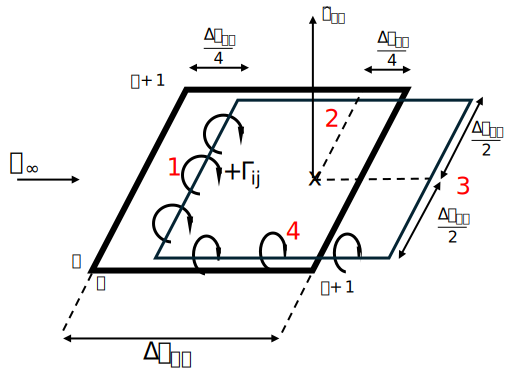
\includegraphics[width=0.8\textwidth]{Quadrilateral vortex ring element.png}
  \caption{Απεικόνιση στοιχείου \textlatin{Vortex Ring Element}}
  \label{fig:VortexRingElement}
\end{figure}



Οι αριθμοί 1 έως 4 στo \autoref{fig:VortexRingElement}, αντιπροσωπεύουν τα τέσσερα πεπερασμένα ευθύγραμμα τμήματα δινών που συνθέτουν το στοιχείο. Η επαγόμενη ταχύτητα του στοιχείου μπορεί να υπολογιστεί χρησιμοποιώντας την εξίσωση \eqref{eq:V12} σε κάθε τμήμα ξεχωριστά. Για ένα αυθαίρετο σημείο στον χώρο $P(x,y,z)$, η επαγόμενη ταχύτητα είναι:

\begin{equation}
{\vec{V}}_{P} = {\vec{V}}_{1} + {\vec{V}}_{2} + {\vec{V}}_{3} + {\vec{V}}_{4}
\end{equation}

Όπου:

\begin{equation}
    \label{eq:Vi}
{\vec{V}}_{i} = \frac{\Gamma}{4\pi}\ \frac{{\vec{r}}_{i,1} \times {\vec{r}}_{i,2}}{\left| {\vec{r}}_{i,1} \times {\vec{r}}_{i,2} \right|}({\vec{r}}_{i,1} - {\vec{r}}_{i,2}) \cdot \left( \frac{{\vec{r}}_{i,1}}{\left| {\vec{r}}_{i,1} \right|} - \frac{{\vec{r}}_{i,2}}{\left| {\vec{r}}_{i,2} \right|} \right)
\end{equation}

Όπως φάινεται στο \autoref{fig:Vortex ring elements in a grid}, αυτά τα στοιχεία ταξινομούνται σε ένα δισδιάστατο πλέγμα για να καλύψουν το σχήμα της ανυψωτικής επιφάνειας. Για να ικανοποιηθεί η συνθήκη \textlatin{Kutta}, η επίδραση της πίσω δίνης της τελευταίας σειράς πάνελ πρέπει να ακυρωθεί. Επομένως, η τελευταία σειρά πάνελ καθώς και όλα τα πάνελ του απόρρου πρέπει να έχουν την ίδια κυκλοφορία $\Gamma$.

\begin{figure}[H]
    \centering
    \includegraphics[width=\textwidth]{vortex ring model.png}
    \caption{\textlatin{Vortex ring elements} σε πλέγμα \cite{katz2001}}
    \label{fig:Vortex ring elements in a grid}
\end{figure}


Ο συντελεστής επιρροής \(\alpha_{ij}\) είναι ουσιαστικά η επαγόμενη ταχύτητα του \textlatin{i}-οστου στοιχείου δίνης με μοναδιαία κυκλοφορία στο \textlatin{j}-οστό σημείο ολοκλήρωσης. Οι συντελεστές επιρροής μπορούν να υπολογιστούν εύκολα χρησιμοποιώντας την εξίσωση \eqref{eq:Vi}. Επαναλαμβάνονας τον υπολογισμό για όλα τα πάνελ και όλα τα σημεία ολοκλήρωσης οδηγεί σε έναν πίνακα.

\begin{equation}
A = \begin{bmatrix}
a_{11} & a_{12} & \cdots & a_{1m} \\
a_{21} & a_{22} & \cdots & a_{2m} \\
 \vdots & \vdots & \ddots & \vdots \\
a_{m1} & a_{m2} & \cdots & a_{mm}
\end{bmatrix}
\end{equation}

\begin{figure}[H]
  \centering
  \includegraphics[width=\textwidth]{2D ARRAY OF PANELS.png}
  \caption{Διάταξη από \textlatin{wing} και \textlatin{wake panels} \cite{katz2001}}
\end{figure}

Για λόγους πληρότητας, το σύνολο των γραμμικών εξισώσεων που πρέπει να λυθεί προκειμένου να υπολογιστεί η ένταση της κυκλοφορίας κάθε στοιχείου για μια δεδομένη γωνία προσβολής για κάθε πάνελ είναι:

\begin{equation}
\begin{bmatrix}
a_{11} & a_{12} & \cdots & a_{1m} \\
a_{21} & a_{22} & \cdots & a_{2m} \\
 \vdots & \vdots & \ddots & \vdots \\
a_{m1} & a_{m2} & \cdots & a_{mm}
\end{bmatrix}\begin{bmatrix}
\Gamma_{1} \\
\Gamma_{2} \\
 \vdots \\
\Gamma_{m}
\end{bmatrix} = \begin{bmatrix}
 - {\vec{Q}}_{\infty} \cdot {\hat{n}}_{1} \\
 - {\vec{Q}}_{\infty} \cdot {\hat{n}}_{2} \\
 \vdots \\
 - {\vec{Q}}_{\infty} \cdot {\hat{n}}_{m}
\end{bmatrix}
\end{equation}


Η καθοδική ροή που προκαλείται σε κάθε στοιχείο δακτυλίου δίνης μπορεί να υπολογιστεί με ένα άλλο σύνολο γραμμικών εξισώσεων.

\begin{equation}
\begin{bmatrix}
{w_{ind}}_{1} \\
{w_{ind}}_{2} \\
 \vdots \\
{w_{ind}}_{m}
\end{bmatrix} = \begin{bmatrix}
b_{11} & b_{12} & \cdots & b_{1m} \\
b_{21} & b_{22} & \cdots & b_{2m} \\
 \vdots & \vdots & \ddots & \vdots \\
b_{m1} & b_{m2} & \cdots & b_{mm}
\end{bmatrix}\begin{bmatrix}
\Gamma_{1} \\
\Gamma_{2} \\
 \vdots \\
\Gamma_{m}
\end{bmatrix}
\end{equation}


Η άντωση και η αντίσταση μπορούν στη συνέχεια να υπολογιστούν χρησιμοποιώντας τις σχέσεις:

\begin{multline}
    L = \sum_{i = 1}^{M} \sum_{j = 1}^{N} \Delta L_{ij}, \\
    \text{Όπου} \quad \Delta L_{ij} = \begin{cases}
      \rho Q_{\infty} \left( \Gamma_{i,j} - \Gamma_{i - 1,j} \right) \Delta y_{ij}, & \text{γιά } i > 1 \\
      \rho Q_{\infty} \Gamma_{ij} \Delta y_{ij}, & \text{γιά } i = 1
    \end{cases}
  \end{multline}

\begin{multline}
D = \sum_{i = 1}^{M} \sum_{j = 1}^{N} \Delta D_{ij}, \\
\text{Όπου} \quad \Delta D_{ij} = \begin{cases}
    \rho w_{\text{ind}_{i,j}} \left( \Gamma_{i,j} - \Gamma_{i - 1,j} \right) \Delta y_{ij}, & \text{γιά } i > 1 \\
    \rho w_{\text{ind}_{i,j}} \Gamma_{ij} \Delta y_{ij}, & \text{γιά } i = 1
\end{cases}
\end{multline}


\section{Εξισώσεις Ανάλυσης Πτερυγισμού}\label{flutter-analysis-equations}

Η γενική μορφή της αεροελαστικής εξίσωσης κίνησης είναι \cite{AeroelasticityWright}

\begin{equation}
    \lbrack A\rbrack\ddot{q} + \left( \rho V\lbrack B\rbrack + D \right)\dot{q} + \left( \rho V^{2}\lbrack C\rbrack + \lbrack E\rbrack \right)q = \lbrack 0\rbrack  
\end{equation}



Όπου:

\begin{itemize}
  \item
    $[A]$, $[C]$, και $[E]$, είναι οι πίνακες που αντιστοιχούν στους $[M]$, $[C]$ και
    $[K]$ που είναι ο κλασικός συμβολισμός που χρησιμοποιείται στην ανάλυση ταλαντώσεων.
  \item
    $[B]$ και $[C]$ είναι οι αεροδυναμικοί πίνακες που εξαρτώνται από τον αριθμό \textlatin{Mach}
    και τη μειωμένη συχνότητα \textlatin{reduced frequency}. Ο τρόπος υπολογισμού αυτών των πινάκων μπορεί να
    ποικίλλει ανάλογα με την αεροδυναμική θεωρία που χρησιμοποιείται.
  \item
    $q$ είναι οι γενικευμένες συντεταγμένες.
  \end{itemize}
  
  


  \subsection{Σύνδεση της κατασκευής με την αεροδυναμική -- \textlatin{ Infinite Plate splines}}\label{interconnection-of-the-structure-with-aerodynamics-infinite-plate-splines}

  Οι  κατασκευαστικοί και οι αεροδυναμικοί βαθμοί ελευθερίας συνδέονται μέσω παρεμβολής. Αυτό επιτρέπει την ανεξάρτητη επιλογή των σημείων πλέγματος (κόμβων) των κατασκευαστικών και αεροδυναμικών πινάκων, αποσυνδέοντας έτσι τις δύο διακριτοποιήσεις της γεωμετρίας. Αυτή η μέθοδος παρεμβολής ονομάζεται \textlatin{splining}. To \textlatin{spline} άπειρης πλάκας που φαίνεται στο \autoref{fig:Surface Spline coordinate system} (\textlatin{Infinite Plate Spline}) και χρησιμοποιείται εδώ, βασίζεται στην παραμόρφωση μιας θεωρητικά άπειρης πλάκας που υπόκειται σε σημειακά φορτία σε συγκεκριμένα σημεία. Τα \textlatin{splines} χρησιμοποιούνται για δύο διαφορετικούς σκοπούς. Ως παρεμβολέας δυνάμεων για τον υπολογισμό της ισοδύναμης κατανομής δυνάμεων στην κατασκευή και ως παρεμβολέας μετατόπισης για τον υπολογισμό ενός συνόλου αεροδυναμικών μετατοπίσεων δεδομένου ενός συνόλου κατασκευαστικών μετατοπίσεων. Μαθηματικά αυτό σημαίνει ότι:
  
  

\begin{equation}
F_{s} = \left\lbrack G_{s \rightarrow a} \right\rbrack F_{a},\ \ U_{a} = {\lbrack G}_{a \rightarrow s}\rbrack U_{s}
\end{equation}


Όπου:

\begin{itemize}
  \item
    $F_{s}$ και $F_{a}$ είναι τα διανύσματα κατασκευαστικών και αεροδυναμικών δυνάμεων.
  \item
    $U_{a}$ και $U_{s}$ είναι τα αεροδυναμικά και κατασκευαστικά διανύσματα μετατόπισης.
  \item
    $G_{s \rightarrow a}$ και $G_{a \rightarrow s}$ είναι οι πίνακες \textlatin{spline} που συνδέουν το κατασκευαστικό με το αεροδυναμικό πρόβλημα και αντίστροφα. Έχει αποδειχθεί με την αρχή του εικονικού έργου ότι ο ένας πίνακας \textlatin{spline} είναι ο ανάστροφος του άλλου. Δηλαδή: 
    $\left\lbrack G_{s \rightarrow a} \right\rbrack = {{\lbrack G}_{a \rightarrow s}\rbrack}^{T}$ .
  \end{itemize}

\begin{figure}[H]
  \centering
  \includegraphics[width=0.9\textwidth]{surface spline.png}
  \caption{Σύστημα συντεταγμένων \textlatin{Surface Spline} \cite{msc2021}}
  \label{fig:Surface Spline coordinate system}
\end{figure}

Το \textlatin{Infinite plate spline} και όλα τα άλλα επιφανειακά \textlatin{splines} χρησιμοποιούνται για να βρουν μια επιφάνεια της μορφής $w(x,y)$ για όλα τα σημεία $(x,y)$ όταν το $w$ είναι
γνωστό σε ένα διακριτό σύνολο σημείων $w_{i} = w\left( x_{i},y_{i} \right)$.

Το \textlatin{Infinite plate spline} μιμείται τη συμπεριφορά μιας άπειρης πλάκας υπό σημειακή φόρτιση. Η παραμόρφωση μιας τέτοιας πλάκας λόγω ενός ενιαίου συγκεντρωμένου φορτίου στο σημείο $\left( x_{i} = 0,\ y_{i} = 0 \right)$ ονομάζεται θεμελιώδης λύση. Η κυβερνητική εξίσωση είναι:



\begin{equation}
D\nabla^{4}(w) = D\frac{1}{r}\frac{d}{dr}\left\{ r\frac{d}{dr}\left\lbrack \frac{1}{r}\frac{d}{dr}\left( r\frac{dw}{dr} \right) \right\rbrack \right\} = q
\label{eq:splineequation}
\end{equation}

Η γενική λύση της ομογενούς μορφής της εξίσωσης \ref{eq:splineequation} είναι:

\begin{equation}
   w = C_{1} + C_{1}r^{2} + C_{2}\ln(r) + C_{3}r^{2}\ln(r) 
\end{equation}

Θέτοντας $C_{2} = \ 0\ $ για να παραμείνει η λύση πεπερασμένη στο $r = 0$, τότε η ολοκλήρωση από το $r = 0$ στο $r = \epsilon\ (small\ number)$ οδηγεί στο $C_{3} = \frac{P}{8\pi D}$. Έτσι, η θεμελιώδης λύση για συγκεντρωμένο φορτίο είναι:

\begin{equation} w = A + Br^{2} + \frac{P}{16\pi D}r^{2}\ln\left( r^{2} \right) \end{equation}

Η θεμελιώδης λύση μπορεί να υπερτεθεί για την επίλυση όλου του προβλήματος της πλάκας:

\begin{equation} w(x,y) = \alpha_{0} + \alpha_{1}x + \alpha_{2}y + \sum_{i = 1}^{N}{K_{i}(x,y)P_{i}} \end{equation}

Όπου:

\begin{itemize}
\item
  $K_{i}(x,y) = \frac{1}{16\pi D}r_{i}^{2}\ln\left( r_{i}^{2} \right)$
\item
  $r_{i}^{2} = \left( x - x_{i} \right)^{2} + \left( y - y_{i} \right)^{2}$
\item
  $P_{i}$ \textlatin{concentrated load at} $\left( x_{i},y_{i} \right)$
\end{itemize}

Οι $N+3$ άγνωστοι καθορίζονται από τις $N+3$ εξισώσεις.

\begin{equation}
\sum_{}^{}{Pi} = 0
\end{equation}

\begin{equation}
  \sum_{}^{}{x_{i}P_{i}} = 0
\end{equation}

\begin{equation}
  \sum_{}^{}{y_{i}P_{i}} = 0
\end{equation}

\begin{equation}
  w_{j} = a_{0} + a_{1}x_{j} + a_{2}y_{2} + \sum_{i = 1}^{N}K_{ij}P_{i},\ \ (\ j = 1,\ldots,\ N)  
\end{equation}

Όπου $K_{ij} = K_{i}\left( x_{j},y_{j} \right)$ καί
$K_{ij} = K_{ji},\ \ K_{ij} = 0\ \text{όταν}\ i = j$

Αυτές οι $N+3$ εξισώσεις μπορούν να εκφραστούν σε μορφή πίνακα:

\begin{equation}
\begin{bmatrix}
  \begin{array}{c}
    0 \\
    0 \\
    0 \\
    \hline
    w_{1} \\
    w_{2} \\
     \vdots \\
    w_{N}        
  \end{array}
\end{bmatrix} = \begin{bmatrix}
\begin{array}{cccccc}
  0 & 0 & 0 & 1 & \cdots & 1 \\
0 & 0 & 0 & x_{1} & \cdots & x_{N} \\
0 & 0 & 0 & y_{1} & \cdots & y_{N} \\
\hline 
1 & x_{1} & y_{1} & 0 & \cdots & K_{1N} \\
1 & x_{2} & y_{2} & K_{21} & \cdots & K_{2N} \\
 \vdots & \vdots & \vdots & \vdots & \cdots & \vdots \\
1 & x_{N} & y_{N} & K_{N1} & \cdots & 0
\end{array}
\end{bmatrix}
\begin{bmatrix}
  \begin{array}{c}
    a_{0} \\
    a_{1} \\
    a_{2} \\
    \hline
    P_{1} \\
    P_{2} \\
     \vdots \\
    P_{N}
        
  \end{array}
\end{bmatrix} = \lbrack C\rbrack\lbrack P\rbrack
\end{equation}

Τώρα που τα $a_{i}$ και $P_{i}$ είναι γνωστά, η παρεμβολή μπορεί να εφαρμοστεί σε οποιοδήποτε μέγεθος για κάθε σημείο στο επίπεδο $(x,y)$ χρησιμοποιώντας την ακόλουθη εξίσωση:

\begin{equation}
\left\{ w \right\} = \begin{bmatrix}
1 & x_{1} & y_{1} & K_{1,1} & K_{1,2} & \cdots & K_{1,n} \\
1 & x_{2} & y_{2} & K_{2,1} & K_{2,2} & \cdots & K_{2.m} \\
 \vdots & \vdots & \vdots & \vdots & \vdots & \cdots & \vdots \\
1 & x_{n} & y_{n} & K_{n,1}\  & K_{n,2} & \cdots & K_{n,n}\ 
\end{bmatrix} \cdot \lbrack C\rbrack^{- 1}\begin{bmatrix}
0 \\
0 \\
0 \\
w_{1} \\
w_{2} \\
 \vdots \\
w_{N}
\end{bmatrix}
\end{equation}

\subsection{Η μέθοδος επίλυσης πτερυγισμού \textlatin{PK}}
\label{the-pk-method-of-flutter-solution}

Η θεμελιώδης εξίσωση για την ανάλυση πτερυγισμού χρησιμοποιώντας τη μέθοδο $PK$ είναι \cite{msc2021}:

\begin{equation}
\left\lbrack M_{hh}p^{2} + \left( B_{hh} - \frac{1}{4}\rho cV\frac{Q_{hh}^{I}}{k} \right)p + \left( K_{hh} - \frac{1}{2}\rho V^{2}Q_{hh}^{R} \right)\  \right\rbrack \cdot \left\{ u_{h} \right\} = \underline{0}
\end{equation}


Όπου:

\begin{itemize} 
  \item $M_{hh} =$ πίνακας μάζας ιδιομορφών, συνήθως διαγώνιος. 
  \item $B_{hh} =$ πίνακας απόσβεσης ιδιομορφών. 
  \item $K_{hh} =$ πίνακας δυσκαμψίας ιδιομορφών, συνήθως διαγώνιος, μπορεί να είναι και μιγαδικός αν χρησιμοποιηθεί πραγματική απόσβεση. 
  \item $Q_{hh}(M,k) =$ πίνακας αεροδυναμικής δύναμης που είναι συνάρτηση του αριθμού $Mach$ και της μειωμένης συχνότητας $k = \frac{\omega\overline{c}}{2V}$.
  \item $Q_{hh}{R}, Q_{hh}{I}$ είναι τα πραγματικά και φανταστικά μέρη του πίνακα αεροδυναμικής δύναμης $Q_{hh}$ ή πίνακες αεροδυναμικής δυσκαμψίας και αεροδυναμικής απόσβεσης αντίστοιχα. 
  \item $k = \frac{\omega\overline{c}}{2V}$ μειωμένη συχνότητα \textlatin{reduced frequency}. 
  \item $M =$ αριθμός $Mach$. 
  \item $V = \ $ ταχύτητα. 
  \item $\rho =$ πυκνότητα ρευστού. 
  \item $\left\{ u_{h} \right\} =$ \textlatin{modal participation vector.}
  \item $p = \omega(\gamma \pm i)$ ιδιοτιμή. 
\end{itemize}


Η εξίσωση επαναδιατυπώνεται στη μορφή \textlatin{state-space} με μείωση τάξης.
\begin{equation}
    \label{eq:PKss}
\lbrack A - pI\rbrack\left\{ {\overline{u}}_{h} \right\} = 0
\end{equation}

Όπου:

\begin{equation}
\lbrack A\rbrack = - \begin{bmatrix}
\mathbf{\lbrack 0\rbrack} & \mathbf{\lbrack I\rbrack} \\
 - M_{hh}^{- 1}\left( K_{hh} - \frac{1}{2}\rho V^{2}Q_{hh}^{R} \right) & - M_{hh}^{- 1}\left( B_{hh} - \frac{1}{4}\rho cV\frac{Q_{hh}^{I}}{k} \right)
\end{bmatrix}
\end{equation}

\begin{equation}
  {\overline{u}}_{h} = \begin{bmatrix}
    u_{h} \\
    {\dot{u}}_{h}
    \end{bmatrix}\  
\end{equation}


Ο βασικός αλγόριθμος για τη μέθοδο $PK$ περιλαμβάνει τα ακόλουθα βήματα:

\begin{enumerate} 
  \def\labelenumi{\arabic{enumi}.} 
  \item Γίνεται μια αρχική εκτίμηση της ιδιοσυχνότητας για την ιδιομορφή. 
  \item Υπολογίζεται η μειωμένη συχνότητα $k$ και η ταχύτητα $V$.
  \item Προσδιορίζονται (με παρεμβολή) οι πίνακες αεροδυναμικής δυσκαμψίας και απόσβεσης $Q_{hh}{R}, Q_{hh}{I}$. 
  \item Προσδιορίζονται οι ιδιοσυχνότητες για το σύστημα σε αυτήν την πτητική συνθήκη χρησιμοποιώντας την εξίσωση \eqref{eq:PKss}. 
  \item Επιλέγεται η ιδιοσυχνότητα που ήταν πιο κοντά στην αρχική εκτίμηση και επαναλαμβάνονται τα βήματα 1-5 μέχρι να συγκλίνει η λύση για τη συχνότητα.
  \item Αποθηκεύεται η τελική ιδιοσυχνότητα και η απόσβεση της ιδιομορφής. 
  \item Εξετάζεται η επόμενη ιδιομορφή ενδιαφέροντος χρησιμοποιώντας την ίδια διαδικασία μέχρι να έχουν διερευνηθεί όλες οι ιδιομορφές. 
\end{enumerate}


\section{Τεχνικές βελτιστοποίησης} \label{optimization-techniques}

\subsection{Μέθοδος γραμμικής αναζήτησης \textlatin{Brent -- Dekker}} \label{brents-dekker-line-search-method}

Αυτός ο αλγόριθμος στοχεύει στην εύρεση του ελαχίστου μιας συνάρτησης μιας μεταβλητής χωρίς τη χρήση των παραγώγων της. Αυτός ο αλγόριθμος χρησιμοποιείται συνήθως για την εύρεση του ελαχίστου μιας συνάρτησης $g\left( \mathbf{x} \right)$ πολλαπλών μεταβλητών \cite{brent1973}. Για το σκοπό αυτό συχνά απαιτείται η ελαχιστοποίηση της ακόλουθης συνάρτησης

\begin{equation}
    \label{eq:minfun}
\gamma(\lambda) = f(\mathbf{x}_{0} + \lambda\mathbf{s})
\end{equation}

Όπου $\mathbf{x}_0$ και $\mathbf{s}$ είναι σταθερά και το $\lambda$ είναι μια βαυμωτή μεταβλητή. Το πρόβλημα αυτό περιγράφει ουσιαστικά μια μονοδιάστατη αναζήτηση ξεκινώντας από το $\mathbf{x}_0$ προς την κατεύθυνση του $\mathbf{s}$.

Ο αλγόριθμος βρίσκει μια προσέγγιση στο ελάχιστο μιας συνάρτησης $f$ ορισμένης στο διάστημα $\lbrack a,\ b\rbrack$. Υπάρχουν έξι σημαντικά σημεία $a,b,u,v,w$ και $x$ τα οποία δεν είναι όλα διακριτά. Μία πιθανή διάταξη των σημείων αυτών φαίνεται στο \autoref{fig:A possible configuration of points}. Αυτά τα σημεία αρχικοποιούνται ως εξής:

\begin{equation}
    \label{eq:brentspoints}
v = w = x = a + \left( \frac{3 - \sqrt{5}}{2} \right)(b - a)
\end{equation}

Ο αριθμός $\left( \frac{3 - \sqrt{5}}{2} \right)$ προέρχεται από τον αλγόριθμο αναζήτησης χρυσής τομής και είναι αυθαίρετη επιλογή. Τα σημεία που ορίζονται στην εξίσωση \eqref{eq:brentspoints} εξυπηρετούν ένα συγκεκριμένο σκοπό:

\begin{itemize} 
  \item Τα σημεία $a$ και $b$ ορίζουν το διάστημα μέσα στο οποίο βρίσκεται ένα τοπικό ελάχιστο. 
  \item $x$: από όλα τα σημεία στα οποία έχει υπολογιστεί η $f$, το $x$ είναι το σημείο με την ελάχιστη τιμή της $f$. 
  \item $w$ είναι το σημείο με την επόμενη χαμηλότερη τιμή του $f$. 
  \item $v$ είναι η προηγούμενη τιμή του $w$. 
  \item $u$ είναι το τελευταίο σημείο στο οποίο έχει υπολογιστεί η $f$.
\end{itemize}

\begin{figure}
  \centering
  \includegraphics[width=\textwidth]{brents_six_points.png}
  \caption{Μια πιθανή διαμόρφωση σημείων  \cite{brent1973} }
  \label{fig:A possible configuration of points}
\end{figure}

Μια τυπική επανάληψη του αλγόριθμου εξελίσσεται ως εξής:


\begin{enumerate} 
  \def\labelenumi{\arabic{enumi}.} 
  \item Έστω $m = 1\text{/}2(a + b)$ το μέσο του διαστήματος.

  \begin{enumerate} \def\labelenumii{\alph{enumii}.} 
      \item Αν $|x - m| \leq 2 \cdot tol - \frac{1}{2}(b - a)\ $, τότε ο αλγόριθμος τερματίζεται με το $x$ ως ελάχιστο. 
      \item Διαφορετικά, οι αριθμοί $p$ και $q$ υπολογίζονται έτσι ώστε $x + p/q$ να είναι το ελάχιστο της παραβολής που διέρχεται από τα σημεία\\ $\left( v,f(v) \right),\ \ \left( w,f(w) \right),\ \ \left( x,f(x) \right)$. 
  \end{enumerate} 

  \item Έστω $e$ η τιμή του $p/q$.
  
  \begin{enumerate} \def\labelenumii{\alph{enumii}.} 
    \item Αν $|e| \leq tol$,\ $q = 0$,\ $x + p\text{/}q \notin \lbrack a,b\rbrack$ ή $\left| p\text{/}q \right| \geq 1/2|e|$, τότε πραγματοποιείται το βήμα της χρυσής τομής:
  
    \begin{equation} u = \begin{cases} \frac{\sqrt{5} - 1}{2}x + \frac{3 - \sqrt{5}}{2}a, & \text{αν } x \geq m \\ \frac{\sqrt{5} - 1}{2}x + \frac{3 - \sqrt{5}}{2}b, & \text{αν } x < m \end{cases} \end{equation}
  
    \item Διαφορετικά $u = x + p\text{/}q$ (οι αποστάσεις $|u - x|,\ \ u - a,\ \ b - u\ $ πρέπει να είναι τουλάχιστον $tol$). 
  \end{enumerate}
\end{enumerate}


\begin{enumerate}
  \def\labelenumi{\arabic{enumi}.}
  \setcounter{enumi}{2}
  \item
    Η $f$ υπολογίζεται στο νέο σημείο $u$ και τα σημεία
    $a,b,v,w\ \text{και}\ x$ ενημερώνονται και ο κύκλος επαναλαμβάνεται.
  \end{enumerate}

  Ο αλγόριθμος συνήθως τερματίζει όταν $x = b - tol$ ή
  $x = a + tol$ μετά από την πραγματοποίηση μιας παραβολικής παρεμβολής, όπου
  έχει εφαρμοστεί η συνθήκη ότι $|u - x| \geq tol$. Το επόμενο
  σημείο παραβολικής παρεμβολής βρίσκεται κοντά στα $x$ και $b$, επομένως το $u$ είναι αναγκαστικά
  $x - tol$. Μια τυπική κατάσταση στην οποία ο αλγόριθμος τερματίζει φαίνεται στο \autoref{fig:typical terminal configuration of important points}

\begin{figure}[H]
    \centering
    \includegraphics[width=\textwidth]{brents algorithm termination configuration.png}
    \caption{Τυπική τερματική διαμόρφωση σημαντικών σημείων \cite{brent1973}}
    \label{fig:typical terminal configuration of important points}

\end{figure}

\subsection{Η Μέθοδος του \textlatin{Powell}}
\label{powells-method}

Η μέθοδος του \textlatin{Powell} είναι μια τροποποιημένη κυκλική αναζήτηση συντεταγμένων. Και οι δύο μέθοδοι στοχεύουν στην ελαχιστοποίηση μιας συνάρτησης πολλών μεταβλητών χωρίς να χρησιμοποιούν καμία από τις παραγώγους της. Γι' αυτό αποκαλούνται μέθοδοι μηδενικής τάξης.

Η μέθοδος κυκλικής αναζήτησης συντεταγμένων είναι στην ουσία μια σειρά βελτιστοποιήσεων γραμμικής αναζήτησης που εκτελούνται κυκλικά σε όλες τις παραμέτρους της συνάρτησης. Η αναζήτηση ξεκινά από ένα αρχικό $x^{(0)}$ και βελτιστοποιεί την πρώτη παράμετρο:

\begin{equation}
\mathbf{x}^{(1)} = \arg_{x_{1}}{\min{f\left( x_{1},x_{2}^{(0)},\ldots,x_{n}^{(0)} \right)}}
\end{equation}

Αφού βρεθεί αυτό, βελτιστοποιεί την επόμενη παράμετρο:

\begin{equation}
\mathbf{x}^{(2)} = \arg_{x_{2}}{\min{f\left( x_{1}^{(1)},x_{2},\ldots,x_{n}^{(1)} \right)}}
\end{equation}

Αυτό μπορεί επίσης να εκφραστεί με τη βοήθεια της εξίσωσης \eqref{eq:minfun} αν $\mathbf{s}$ είναι το \textlatin{i}-οστό διανύσμα βάσης για $i = 1,\ldots,n$.

Μπορεί να χρησιμοποιηθεί οποιοσδήποτε αλγόριθμος γραμμικής αναζήτησης, αλλά ο αλγόριθμος του \textlatin{Brent} βρίσκει ευρεία χρήση σε βιβλιοθήκες βελτιστοποίησης, συμπεριλαμβανομένης της υλοποίησης της μεθόδου \textlatin{Powell} στήν  \textlatin{SciPy}.

\begin{figure}[H]
    \centering
    \includegraphics[width=0.5\textwidth]{cyclic coordinate search.png}
    \caption{Η μέθοδος \textlatin{Cyclic Coordinate Search \cite{kochenderfer2019}}}
    \label{fig:CCsearch}
\end{figure}

Όπως φαίνεται στo \autoref{fig:CCsearch}, ένα μειονέκτημα αυτής της μεθόδου είναι η αργή
προσπέλαση των διαγώνιων κοιλάδων, όπου γίνονται επαναλαμβανόμενα μικρά βήματα σε
κάθε κατεύθυνση. Η ιδέα του \textlatin{M.J.D. Powell} ήταν να επεκτείνει την κυκλική
αναζήτηση συντεταγμένων ώστε να μπορεί να αναζητά σε κατευθύνσεις που
δεν είναι κάθετες μεταξύ τους και ούτε τα διανύσματα βάσης. Για να
επιτευχθεί αυτή η νέα ικανότητα, ο αλγόριθμος του \textlatin{Powell} διατηρεί μια λίστα
κατευθύνσεων αναζήτησης
$\left\lbrack \mathbf{u}^{(0)},\ldots\mathbf{u}^{(n)} \right\rbrack$
οι οποίες αρχικά είναι τα διανύσματα βάσης συντεταγμένων
$\mathbf{u}^{(i)}=\mathbf{e}^{\left( \mathbf{i} \right)}$ για
όλα τα $i$.

Ξεκινώντας από το $\mathbf{x}^{(0)}$, η μέθοδος του \textlatin{Powell} διεξάγει μια γραμμική αναζήτηση όπως και πριν, για κάθε κατεύθυνση αναζήτησης διαδοχικά:


\begin{equation}
\mathbf{x}^{(i + 1)} \leftarrow linesearch\left( f,\mathbf{x}^{(i)}\mathbf{,}\mathbf{u}^{(i)} \right)\mathbf{\ }for\ i\ in\ \lbrack 0,\ldots,n\rbrack
\end{equation}

Στη συνέχεια, όλες οι κατευθύνσεις αναζήτησης μετατοπίζονται κατά έναν δείκτη,
απορρίπτοντας την παλαιότερη κατεύθυνση αναζήτησης, $\mathbf{u}^{(0)}\ $

\begin{equation}
\mathbf{u}^{(i)} \leftarrow \mathbf{u}^{(i + 1)}\ for\ i\ in\ \lbrack 0,\ldots,n - 1\rbrack
\end{equation}

Η τελευταία κατεύθυνση αναζήτησης αντικαθίσταται με την κατεύθυνση από
το $\mathbf{x}^{(0)}$ στο $\mathbf{x}^{(n + 1)}$, που είναι η συνολική
κατεύθυνση της προόδου κατά τις τελευταίες $n$ γραμμικές αναζητήσεις:

\begin{equation}
\mathbf{u}^{(n)} \leftarrow \mathbf{x}^{(n + 1)} - \mathbf{x}^{(0)}
\end{equation}

Αυτή η διαδικασία επαναλαμβάνεται μέχρι τη σύγκλιση.
\begin{figure}[H]
    \centering
    \includegraphics[width=0.5\textwidth]{powells method.png}
    \caption{Η μέθοδος \textlatin{Powell} \cite{kochenderfer2019}}
    \label{fig:Powell}

\end{figure}

Όπως φαίνεται στο \autoref{fig:Powell}, η μέθοδος του Powell ξεκινά όπως η κυκλική
αναζήτηση συντεταγμένων αλλά σταδιακά ((μαθαίνει)) την κατεύθυνση μέγιστης καθόδου.


\subsection{Γενετικός Αλγόριθμος}
\label{genetic-algorithm}

Οι γενετικοί αλγόριθμοι μιμούνται τη λογική της Δαρβινικής εξέλιξης, όπου τα
καταλληλότερα ((άτομα)) είναι πιο πιθανό να μεταβιβάσουν τα γονίδιά τους στην επόμενη
γενιά. Τα χρωμοσώματα κάθε ατόμου ορίζουν ένα μόνο σημείο σχεδίασης. Σε κάθε γενιά, τα χρωμοσώματα των καταλληλότερων ατόμων μεταβιβάζονται στην επόμενη γενιά αφού περάσουν απο τα στάδια της \emph{διασταύρωσης, (\latintext{crossover})}  και της \emph{μετάλλαξης, \latintext(mutation)}.

Τα χρωμοσώματα συχνά αναπαρίστανται από ένα λογικό πίνακα, αλλά σε αυτήν την περίπτωση ένας πίνακας πραγματικών τιμών περιγράφει καλύτερα το χώρο σχεδίασης.

\subsubsection{Αρχικοποίηση}

Ο Γενετικός Αλγόριθμος ξεκινά με την αρχικοποίηση ενός πληθυσμού με τυχαία χρωμοσώματα.

\subsubsection{Επιλογή Γονέων}

Η διαδικασία επιλογής είναι η διαδικασία επιλογής των χρωμοσωμάτων που θα δημιουργήσουν απογόνους για την επόμενη γενιά μετά από την υποβολή στις γενετικές διαδικασίες της διασταύρωσης και της μετάλλαξης. Υπάρχουν πολλές μέθοδοι επιλογής των ατόμων που θα ζευγαρώσουν και θα συνδυάσουν τα γονίδιά τους. Μερικές από τις πιο δημοφιλείς περιλαμβάνουν:

\begin{itemize}
\item
  \textlatin{Roulette Wheel selection:} Όπου στο κάθε άτομο έχει ανατεθεί μέρος της
  φανταστικής ρουλέτας ανάλογη με την απόδοσή τους. Στη συνέχεια, η ρουλέτα
  περιστρέφεται μέχρι να επιτευχθεί ο επιθυμητός αριθμός γονέων. Αυτή η μέθοδος είναι
  απλή και αποτελεσματική στις περισσότερες περιπτώσεις. Μπορεί να επηρεαστεί ωστόσο από
  άτομα που είναι πολύ αποδοτικότερα από τον υπόλοιπο πληθυσμό.
\item
  \textlatin{Tournament Selection}: Ένα υποσύνολο ατόμων επιλέγεται τυχαία
  και το καλύτερο άτομο από αυτά επιλέγεται ως γονέας. Η
  διαδικασία επαναλαμβάνεται μέχρι να επιτευχθεί ο επιθυμητός αριθμός γονέων.
\item
\textlatin{Steady State Crossover}: Ένα σταθερό μέρος του πληθυσμού αντικαθίσταται
  σε κάθε γενιά. Μόνο τα αδύναμα άτομα αντικαθίστανται από
  απογόνους, αυτή η μέθοδος διασφαλίζει ότι το καταλληλότερο άτομο
  διατηρείται τις περισσότερες φορές. Ένα μειονέκτημα αυτής της μεθόδου είναι ότι αργεί να προσαρμοστεί, καθώς μόνο ένα μικρό μέρος του πληθυσμού αντικαθίσταται σε κάθε γενιά.
\end{itemize}

\subsubsection{\textlatin{Crossover}}

Η διασταύρωση (\textlatin{Crossover}) είναι ο τρόπος με τον οποίο τα χρωμοσώματα των γονέων συνδυάζονται για
τη δημιουργία απογόνων. Υπάρχουν διάφοροι τρόποι διασταύρωσης. Οι πιο
κοινώς χρησιμοποιούμενοι είναι:
\begin{samepage}
\begin{itemize}
\item
\textlatin{Single point crossover}

Με αυτόν τον τρόπο, το πρώτο τμήμα του χρωμοσώματος του γονέα A σχηματίζει το πρώτο τμήμα του χρωμοσώματος του παιδιού και το τελευταίο τμήμα του χρωμοσώματος του γονέα B σχηματίζει το τελευταίο τμήμα του χρωμοσώματος του παιδιού. Η διαδικασία αυτή φάινεται στο \autoref{fig:Single Point Crossover}


\begin{figure}[H]
    \centering
    \includegraphics[width=\textwidth]{single point crossover.png}
    \caption{Διασταύρωση \textlatin{(Crossover)} ενός σημείου \cite{kochenderfer2019}}
    \label{fig:Single Point Crossover}


\end{figure}


\item
\textlatin{Two point crossover}

Όπως πριν, αλλά όπως φαίνεται στο \autoref{fig:Two-point Crossover} προστίθεται ένα δεύτερο σημείο διασταύρωσης.


\begin{figure}[H]
    \centering
    \includegraphics[width=\textwidth]{two point crossover.png}
    \caption{Διασταύρωση \textlatin{(Crossover)} δύο σημείων \cite{kochenderfer2019}}
    \label{fig:Two-point Crossover}


\end{figure}

\item
\textlatin{Uniform crossover}

Κατά αυτόν τον τρόπο, όπως φάινεται στο \autoref{fig:Uniform Crossover} κάθε χρωμόσωμα έχει 50\% πιθανότητα να προέρχεται από τον γονέα A ή τον γονέα B.

\begin{figure}[H]
    \centering
    \includegraphics[width=\textwidth]{uniform crossover.png}
    \caption{Ομοιόμορφη διασταύρωση \textlatin{(Uniform Crossover) \cite{kochenderfer2019}}}
    \label{fig:Uniform Crossover}

\end{figure}
\end{itemize}
\end{samepage}

\subsubsection{\textlatin{Mutation}}

Η μετάλλαξη είναι ένα απαραίτητο βήμα του γενετικού αλγορίθμου, καθώς επιτρέπει την ανάπτυξη νέων χαρακτηριστικών που δεν υπήρχαν στον αρχικό πληθυσμό. Στην ουσία, μια τυχαία τιμή προστίθεται σε ένα τυχαίο χρωμόσωμα ενός τυχαία επιλεγμένου απογόνου. Η πιθανότητα να συμβεί μια μετάλλαξη σε ένα άτομο ονομάζεται \textlatin{\emph{mutation rate}}.

\subsubsection{\textlatin{Elitism}}

Ο ελιτισμός είναι μια στρατηγική που διασφαλίζει ότι ένας σταθερός αριθμός των καταλληλότερων
ατόμων επιβιώνει στην επόμενη γενιά.

Οι γενετικοί αλγόριθμοι έχουν ένα πολύ ευρύ φάσμα εφαρμογών και είναι πολύ προσαρμόσιμοι σε πολλά προβλήματα. Όμως υπάρχει ένα πρόβλημα. Όλες αυτές οι παράμετροι και στρατηγικές επηρεάζουν σημαντικά τα αποτελέσματα και δεν υπάρχει καμία τυπική μέθοδος επιλογής κάθε παραμέτρου. Επομένως, είναι ευθύνη του ερευνητή να κατανοήσει το πρόβλημα και μέσω πειραματισμού και τεχνικών ρύθμισης υπερπαραμέτρων μοντέλου, να καθορίσει ένα
αρκετά καλό σύνολο παραμέτρων.

\subsection{Νευρωνικά Δίκτυα}
\label{neural-networks}

\subsubsection{Τι είναι τα Τεχνητά Νευρωνικά Δίκτυα \textlatin{(ANN's)}}

Ένα τεχνητό νευρωνικό δίκτυο είναι ένα υπολογιστικό μοντέλο που εμπνέεται από τον τρόπο λειτουργίας του βιολογικού εγκεφάλου. Η βασική δομή ενός \textlatin{ANN} αποτελείται από διασυνδεδεμένους κόμβους (ή νευρώνες) οργανωμένους σε στρώματα.

Η βασική μονάδα αυτής της δομής είναι ο νευρώνας, μια απεικόνιση του οποίου φαίνεται	στο \autoref{fig:The Structure of a Neuron} . Ένας νευρώνας έχει πολύ απλή δομή. Δέχεται έναν αυθαίρετο αριθμό εισόδων μαζί με μια σταθερά προσαύξησης (\textlatin{bias}) και έχει μόνο μία έξοδο. Η έξοδος μπορεί να είναι λογική ή πραγματική. Εντός του νευρώνα, πραγματοποιείται ένα άθροισμα χρησιμοποιώντας το βάρος κάθε εισόδου και την σταθερά προσαύξησης. Το αποτέλεσμα κάθε αθροίσματος επεξεργάζεται περαιτέρω μέσω μιας ((συνάρτησης ενεργοποίησης)) (\textlatin{activation function}) και προκύπτει η έξοδος. Η συνάρτηση ενεργοποίησης επιτρέπει τη μη γραμμική συμπεριφορά των νευρωνικών δικτύων. Μπορεί να είναι οποιαδήποτε συνάρτηση, αλλά ορισμένες συναρτήσεις έχουν επικρατήσει.

\begin{figure}[H]
    \centering
    \includesvg[width=\textwidth]{Neuron.svg}
    \caption{Η δομή ενός νευρώνα}
    \label{fig:The Structure of a Neuron}
    

\end{figure}


Η βασική αρχιτεκτονική ενός νευρωνικού δικτύου φαίνεται στο \autoref{fig:Structure of a Neural Network} και  αποτελείται από:

\begin{enumerate}
\def\labelenumi{\arabic{enumi}.}
\item
  Ένα στρώμα εισόδου το οποίο είναι υπεύθυνο για τη λήψη των αρχικών δεδομένων. 
  Κάθε νευρώνας στο στρώμα εισόδου αντιπροσωπεύει ένα συγκεκριμένο χαρακτηριστικό των δεδομένων εισόδων.
\item
  Κρυφά στρώματα, τα οποία είναι ενδιάμεσα στρώματα μεταξύ των στρωμάτων εισόδου και
  εξόδου και είναι υπεύθυνα για την αναγνώριση σύνθετων χαρακτηριστικών.
\item
  Τα βάρη και οι σταθερές προσαύξησης που χρησιμοποιούνται στο νευρωνικό δίκτυο, και τα οποία είναι οι παράμετροι που πρέπει να εκπαιδευτούν για να μπορέσει το νευρωνικό δίκτυο
  να κάνει ουσιαστικές προβλέψεις.
\item
  Ένα στρώμα εξόδου το οποίο παράγει τις τελικές προβλέψεις. Η έξοδος μπορεί
  να είναι δυαδική για προβλήματα ταξινόμησης ή κλιμακωτή για προβλήματα παλινδρόμησης.
\end{enumerate}

\begin{figure}[H]
    \centering
    \includesvg[width=\textwidth]{Neural Network.svg}
    \caption{Η δομή ενός νευρωνικού δικτύου \cite{takyar2025}}
    \label{fig:Structure of a Neural Network}


\end{figure}

Ο αριθμός των κρυφών στρωμάτων σε ένα νευρωνικό δίκτυο μπορεί να διαφέρει. Τα νευρωνικά δίκτυα που δεν έχουν κρυφά στρώματα ονομάζονται Ρηχά (\textlatin{shallow}), ενώ τα νευρωνικά δίκτυα με κρυφά στρώματα ονομάζονται Βαθιά Νευρωνικά Δίκτυα \textlatin{(Deep Neural Networks)}.


\subsubsection{Εκπαίδευση Τεχνητών Νευρωνικών Δικτύων}

Όπως αναφέρθηκε προηγουμένως, για να είναι χρήσιμο ένα νευρωνικό δίκτυο πρέπει να εκπαιδευτεί. Η εκπαίδευση περιλαμβάνει τη συλλογή δεδομένων παρόμοιων με αυτά που το \textlatin{ΝΝ} προορίζεται να προβλέψει, και την εκτέλεση μιας βελτιστοποίησης των βαρών και των προσαυξήσεων εντός του δικτύου για την ελαχιστοποίηση κάποιας συνάρτησης απώλειας \textlatin{loss function}. Μια συνάρτηση απώλειας είναι ένα μέτρο του ποσού του σφάλματος πρόβλεψης. Υπάρχουν πολλές συναρτήσεις απώλειας που χρησιμοποιούνται συνήθως για τα νευρωνικά δίκτυα, αλλά όταν ένα νευρωνικό δίκτυο εκπαιδεύεται σε ένα πρόβλημα παλινδρόμησης, η συνάρτηση απώλειας είναι συνήθως μία από τις ακόλουθες:

\foreignlanguage{english}{
\begin{enumerate}
\def\labelenumi{\arabic{enumi}.}
\item
  Mean Squared Error (MSE)
\end{enumerate}

\begin{equation}
MSE = \frac{1}{N}\sum_{i = 1}^{N}\left( y_{i} - \hat{y} \right)^{2}
\end{equation}


\begin{enumerate}
\def\labelenumi{\arabic{enumi}.}
\setcounter{enumi}{1}
\item
  Root Mean Squared Error
\end{enumerate}

\begin{equation}
RMSE = \ \sqrt{MSE} = \sqrt{\frac{1}{N}\sum_{i = 1}^{N}\left( y_{i} - \hat{y} \right)^{2}}
\end{equation}

\begin{enumerate}
\def\labelenumi{\arabic{enumi}.}
\setcounter{enumi}{2}
\item
  Mean Average Error (MAE)
  
  \begin{equation}
    MAE = \frac{1}{N}\sum_{i = 1}^{N}{|y_{i} - \hat{y}|}
    \label{eq:MAE}
  \end{equation}
  \textgreek{Όπου: $\hat{y}$ είναι η προβλεπόμενη τιμή του $y$}
\end{enumerate}
}

O στόχος της εκπαίδευσης του νευρωνικού δικτύου είναι η ελαχιστοποίηση οποιασδήποτε από αυτές τις συναρτήσεις στα δεδομένα δοκιμής που το δίκτυο δεν έχει ξαναδεί.

Για να επιτευχθεί αυτός ο στόχος, πρώτα τα διαθέσιμα δεδομένα που περιέχουν τόσο την είσοδο όσο και την επιθυμητή έξοδο, χωρίζονται τυχαία σε δεδομένα εκπαίδευσης (\textlatin{training data}) (αυτά που θα χρησιμοποιηθούν για την προσαρμογή των βαρών και των προσαυξήσεων) και δεδομένα δοκιμής (\textlatin{test data}) (αυτά που θα χρησιμοποιηθούν για την αξιολόγηση της απόδοσης του νευρωνικού δικτύου). Στη συνέχεια, μέσω μιας διαδικασίας που ονομάζεται \textlatin{backpropagation} (η ακριβής εξήγηση της οποίας είναι πέρα από το πεδίο αυτής της διατριβής) σε παρτίδες των δεδομένων εκπαίδευσης, τα βάρη ενημερώνονται με τέτοιο τρόπο ώστε να μειωθεί η τιμή της συνάρτησης απώλειας για αυτό το συγκεκριμένο σύνολο δεδομένων. Μόλις όλες οι παρτίδες δεδομένων έχουν περάσει από το δίκτυο και τα βάρη έχουν προσαρμοστεί ανάλογα, λέμε ότι το δίκτυο έχει ολοκληρώσει ένα πέρασμα μέσω των δεδομένων εκπαίδευσης. Αυτή η διαδικασία εκτιμά την κλίση της συνάρτησης απώλειας και έτσι το δίκτυο κατεβαίνει προς το ελάχιστο της συνάρτησης απώλειας. Ο αριθμός των επαναλήψεων αυτής της διαδικασίας ονομάζεται \textlatin{epochs}. Ο αριθμός των \textlatin{epochs} πρέπει να είναι τέτοιος ώστε να επιτευχθεί μια βέλτιστη λύση χωρίς την υπερπροσαρμογή \textlatin{(overfitting)} του δικτύου στα δεδομένα εκπαίδευσης.

\subsubsection{\textlatin{Hyperparameter Tuning}}

Όπως έχουμε δει, για να ορίσουμε ένα νευρωνικό δίκτυο, πρέπει να επιλέξουμε πολλές παραμέτρους εκ των προτέρων. Αυτές οι παράμετροι περιλαμβάνουν τον αριθμό των κρυφών στρωμάτων, τον αριθμό των νευρώνων σε κάθε στρώμα, και τη συνάρτηση ενεργοποίησης κάθε στρώματος,καθώς και πολλές άλλες. Το βέλτιστο σύνολο παραμέτρων δεν είναι γνωστό εκ των προτέρων και δεν υπάρχει μέθοδος επιλογής του.

Η διαδικασία βελτιστοποίησης των υπερπαραμέτρων ενός μοντέλου ονομάζεται \emph{\textlatin{Hyperparameter Tuning}}. Υπάρχουν πολλοί αλγόριθμοι βελτιστοποίησης που το επιτυγχάνουν αυτό. Ένας από τους πιο ενδιαφέροντες και αυτός που θα χρησιμοποιηθεί για αυτή την εφαρμογή είναι ο αλγόριθμος \textlatin{HyperBand} \cite{li2018hyperbandnovelbanditbasedapproach}. Ο αλγόριθμος αυτός είναι μια βελτίωση του αλγόριθμου \textlatin{Successive Halving}.

Η ιδέα πίσω από τον αλγόριθμο \textlatin{Successive Halving} είναι αρκετά απλή. Κατανέμει ομοιόμορφα έναν προϋπολογισμό πόρων (υπολογιστικού χρόνου) σε ένα σύνολο υπερπαραμέτρων, αξιολογεί την απόδοση κάθε σετ υπερπαραμέτρων, απορρίπτει το χειρότερο 50\% και επαναλαμβάνει μέχρι να απομείνει ένα μόνο σετ υπερπαραμέτρων. Το πρόβλημα με αυτόν τον αλγόριθμο είναι ότι δεν είναι γνωστό εάν η δοκιμή ενός μεγαλύτερου αριθμού διαμορφώσεων με περιορισμένους υπολογιστικούς πόρους η καθεμία ή ενός μικρότερου αριθμού διαμορφώσεων με περισσότερους πόρους, θα έχει καλύτερο αποτέλεσμα.

Αυτό είναι το πρόβλημα που αντιμετωπίζει ο αλγόριθμος \textlatin{HyperBand}. Η αντιμετώπιση επιτυγχάνεται πραγματοποιώντας ένα \textlatin{grid search} για τις εφικτές τιμές των $n$ και $r$, όπου $n$ είναι ο αριθμός των διαμορφώσεων που θα δοκιμαστούν και $r$ είναι η ελαχιστη ποσότητα υπολογιστικής ισχύος που κατανέμεται σε όλες τις διαμορφώσεις πρωτού δύναται να απορριφθούν.

